\documentclass[10pt]{IEEEtran}

\title{Applying The SURF Algorithm to Prokudin-Gorskii Image Sets}
\author{Jeffrey-David Kapp, Sebastian Lenartowicz, and Vincent Yong
\linebreak
\today}

\usepackage{listings}
\lstset{  language=Python, basicstyle=\footnotesize\ttfamily }

\usepackage{graphicx}
\usepackage[section]{placeins}

\begin{document}
\maketitle



\section{SURF}

\subsection{The Algorithm}

The algorithm used to composite the Prokudin-Gorskii images is the "speeded up robust features" (SURF), a feature detector and descriptor commonly used in object recognition, image registration, and image classification. SURF operates three main parts, detection, description, and matching.
\linebreak

In general, each componant functions as follows: SURF feature detection uses the determinate of a Hessian matrix. Points on the image where this determinate is amongst the highest are chosen as "keypoints". SURF's image descriptor first determines the reproducable orientations of the chosen keypoints, then builing a square region aligned with it orientation, and a descriptor is built using the sums of several levels of Haar wavelets. Matching is done by finding matching pairs of descriptors in several images. 

\subsection{Our Implementation}

Implementation is done via OpenCV's implementation of the SURF algorithm. What follows is a description of how OpenCV was used to composite Prokudin-Gorskii images.

All source code is drawn from surf.py found in the submission directory. 

\begin{lstlisting}
imgR = cv2.imread(os.path.join(targetDir, 'r.tif'), 0)
imgG = cv2.imread(os.path.join(targetDir, 'g.tif'), 0)
imgB = cv2.imread(os.path.join(targetDir, 'b.tif'), 0)
bad = np.dstack((imgR, imgG, imgB))

height, width = imgR.shape[:2]
shape = (width, height)
\end{lstlisting}

This part is reading in the .tif images corresponding to Red, Green, and Blue and doing a rough composition that has not been aligned at all. Examples of these images will be included in the experiment examples. R, G, and B are in seperate files as each image has been segmented by hand. Each image is also exactly the same size. 

\begin{lstlisting}
surf = cv2.xfeatures2d.SURF_create()

kpR, desR = surf.detectAndCompute(imgR, None)
kpG, desG = surf.detectAndCompute(imgG, None)
kpB, desB = surf.detectAndCompute(imgB, None)

bf = cv2.BFMatcher(cv2.NORM_L2, crossCheck=False)
\end{lstlisting}

This is the invocation of the SURF algorithm. It will detect and build the discriptors of key points one each of the R, G, and B image, and store the key points themselves in kpX and descriptors in desX. bf is simply a brute force matcher that OpenCV provides. 

\begin{lstlisting}
matches = bf.match(desR, desG)
goodMatches = [m for m in matches if m.distance <= 0.10]
matchR = np.array([kpR[m.queryIdx].pt for m in goodMatches])
matchG = np.array([kpG[m.trainIdx].pt for m in goodMatches])
rgH, mask = cv2.findHomography(matchG, matchR, cv2.RANSAC)
\end{lstlisting}

This code snippet first matches the descriptors of key points in the Red and Green images. It discards all matches that are shifted from one another by more than 10\% of the image's total size. It segregates the matched keypoints by the origin image, and then uses this array of keypoints to find the homography of the keypoints using the RANSAC method. It then does all of this again but for Red and Blue images.  

\begin{lstlisting}
warpG = cv2.warpPerspective(imgG, rgH, shape)
warpB = cv2.warpPerspective(imgB, rbH, shape)

stacked = np.dstack((imgR, warpG, warpB))
\end{lstlisting}

New images are then created for Green and Blue which have been aligned with the keypoints of the Red image. These are then composited together for the final image. 

\section{Experiments}

10, 11, 26, 31, 111, 152, 223, 384(failed)

The following are 8 example images from our testing of SURF's applicability to processing Prokudin-Gorskii images. testing was done with a total of 65 images, these 8 best exemplify the effectiveness and potential failure of SURF in composing images. Each origin image set can be found in it's respective directory in a .tif, along with the r, b, and g segmentation, and the rough and SURF aligned compositions called "original" and "composite" respectively. The origin image sets will not be included in this report, just the rough and aligned composites. 

Images will begin on the next page.
\newpage

\begin{figure}[!htb]
\caption{Rough Composite 00010a}
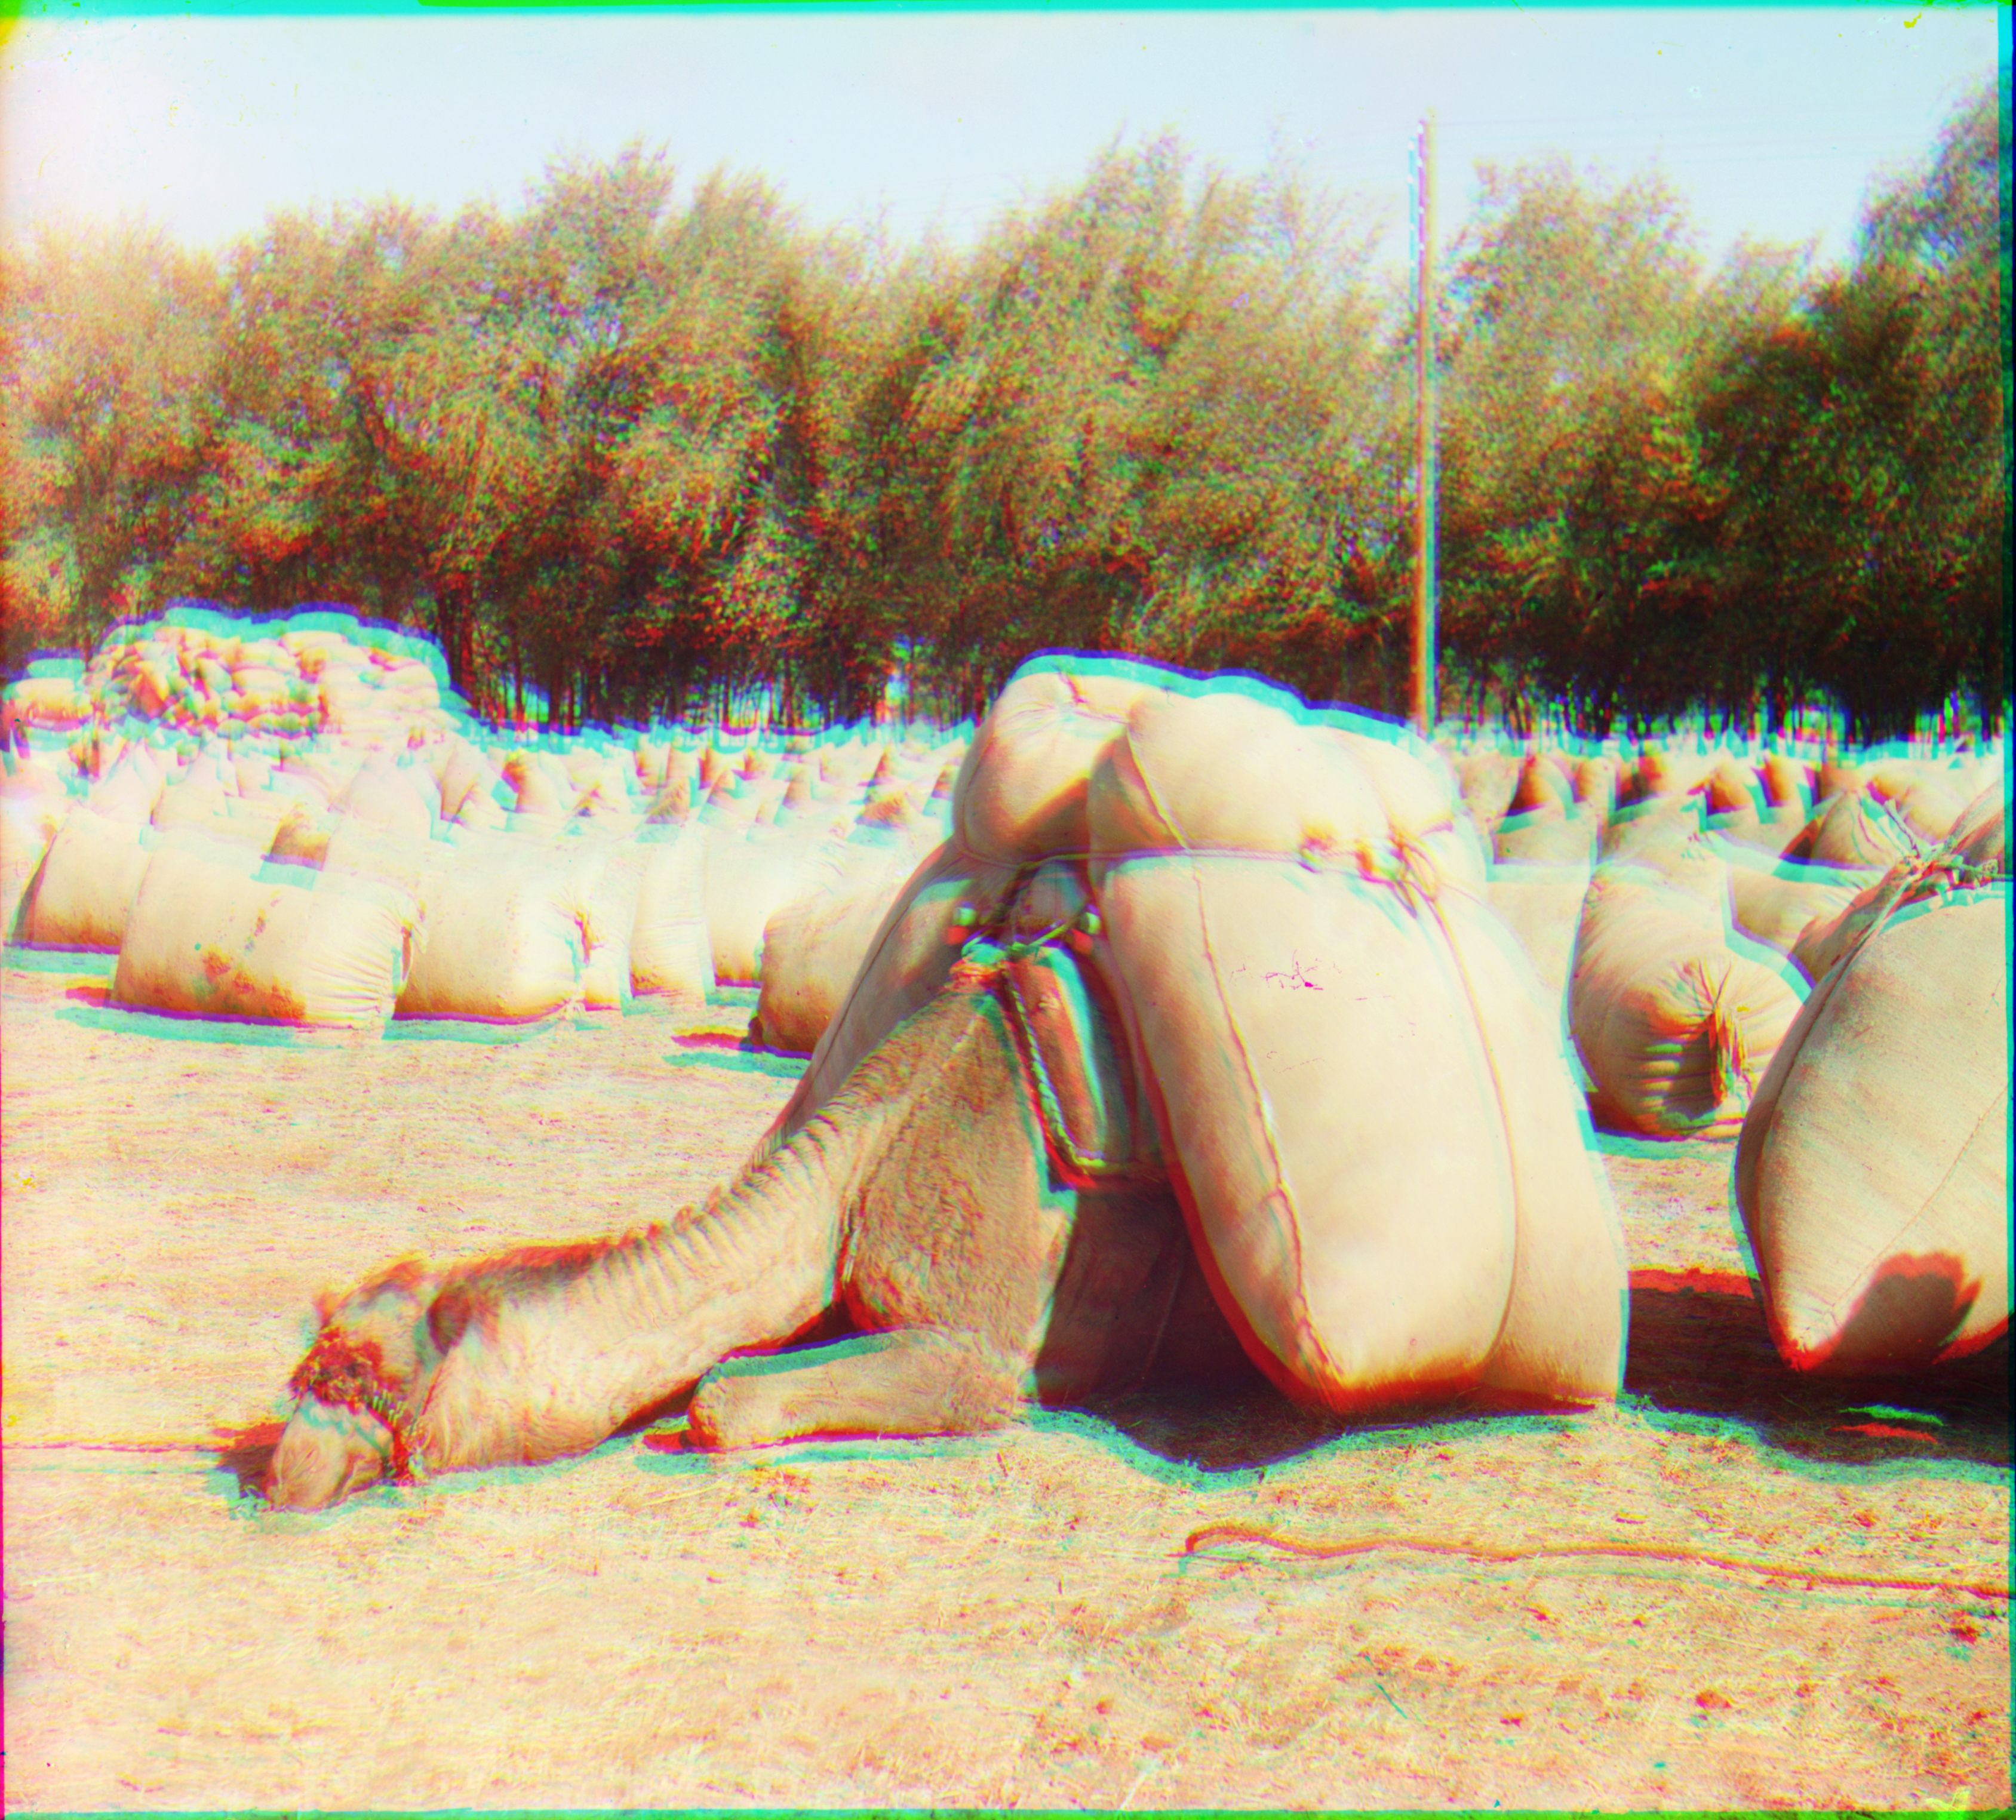
\includegraphics[scale=0.07]{../00010a/original}
\end{figure}

\begin{figure}[!htb]
\caption{SURF Aligned Composite 00010a}
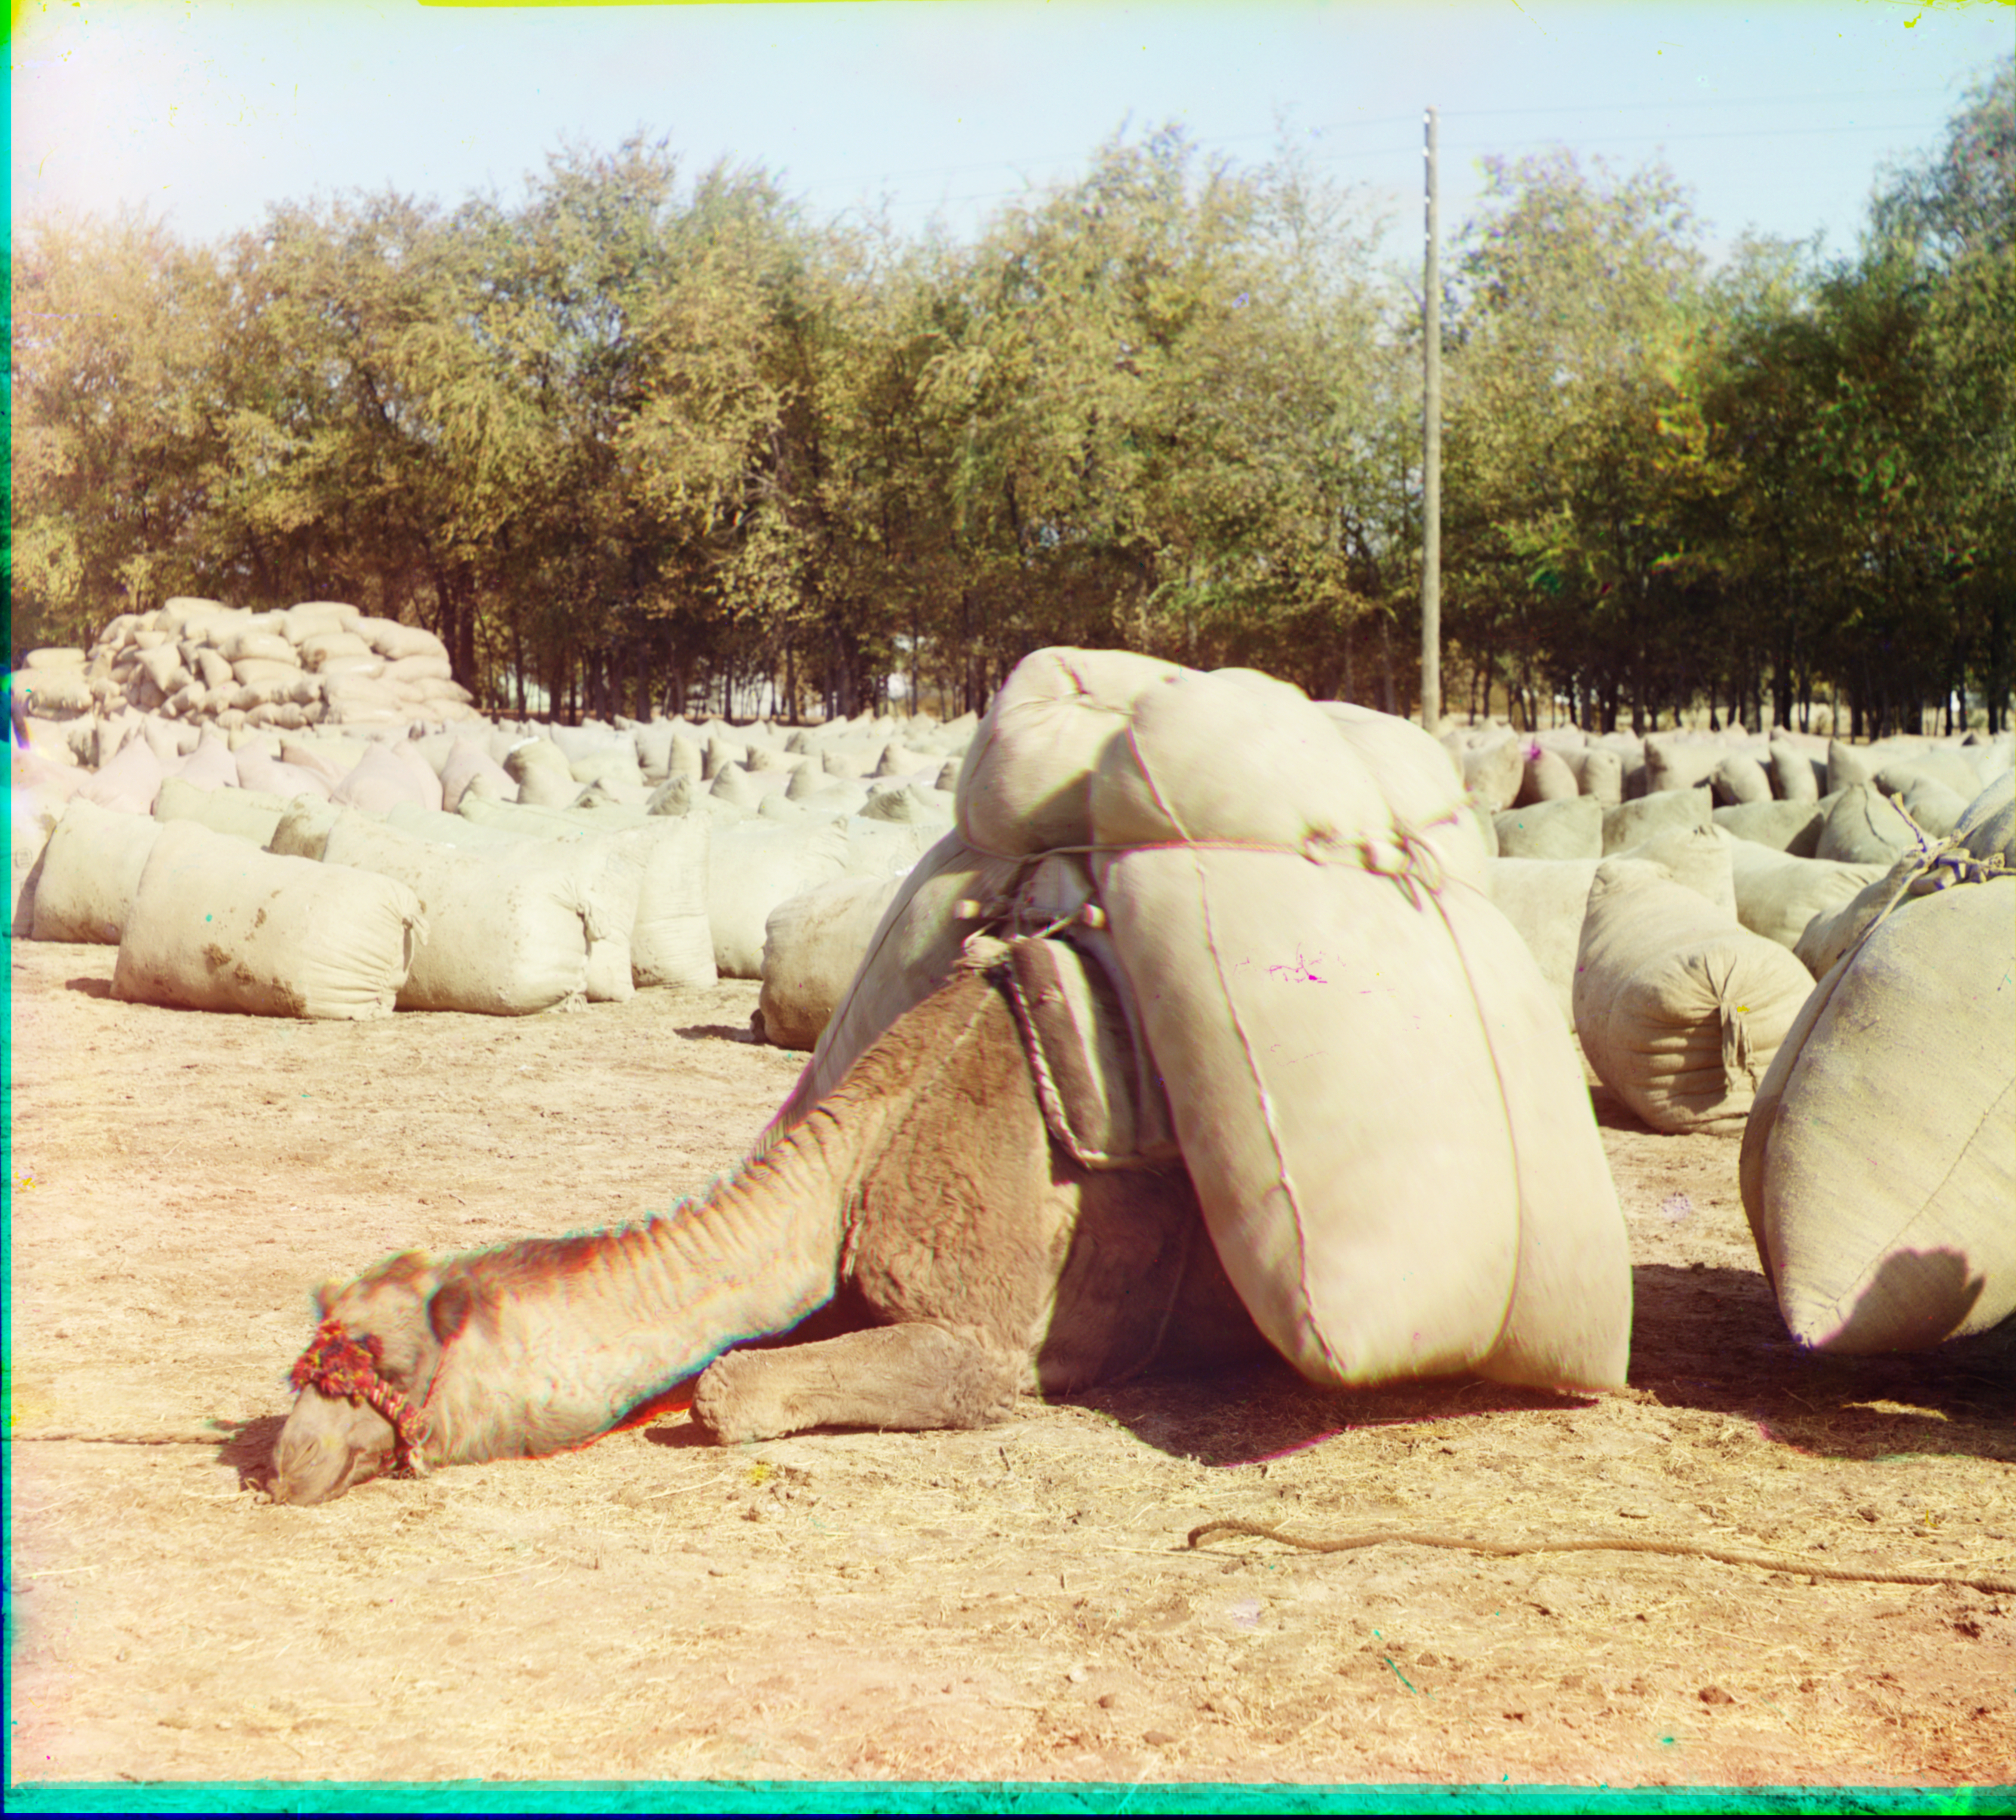
\includegraphics[scale=0.07]{../00010a/composite}
\end{figure}

Here, the offset of the green image can be seen in the rough composite, mainly underneath each of the bags and the camel. The SURF aligned images have mostly elimated these, except about mid way through the camel's neck, and the large green bar at the bottom. Coloured bars like this are caused by the shifting of the Green and Blue images, and will be a common feature in all of the aligned images.

\FloatBarrier

\begin{figure}[!htb]
\caption{Rough Composite 00011a}
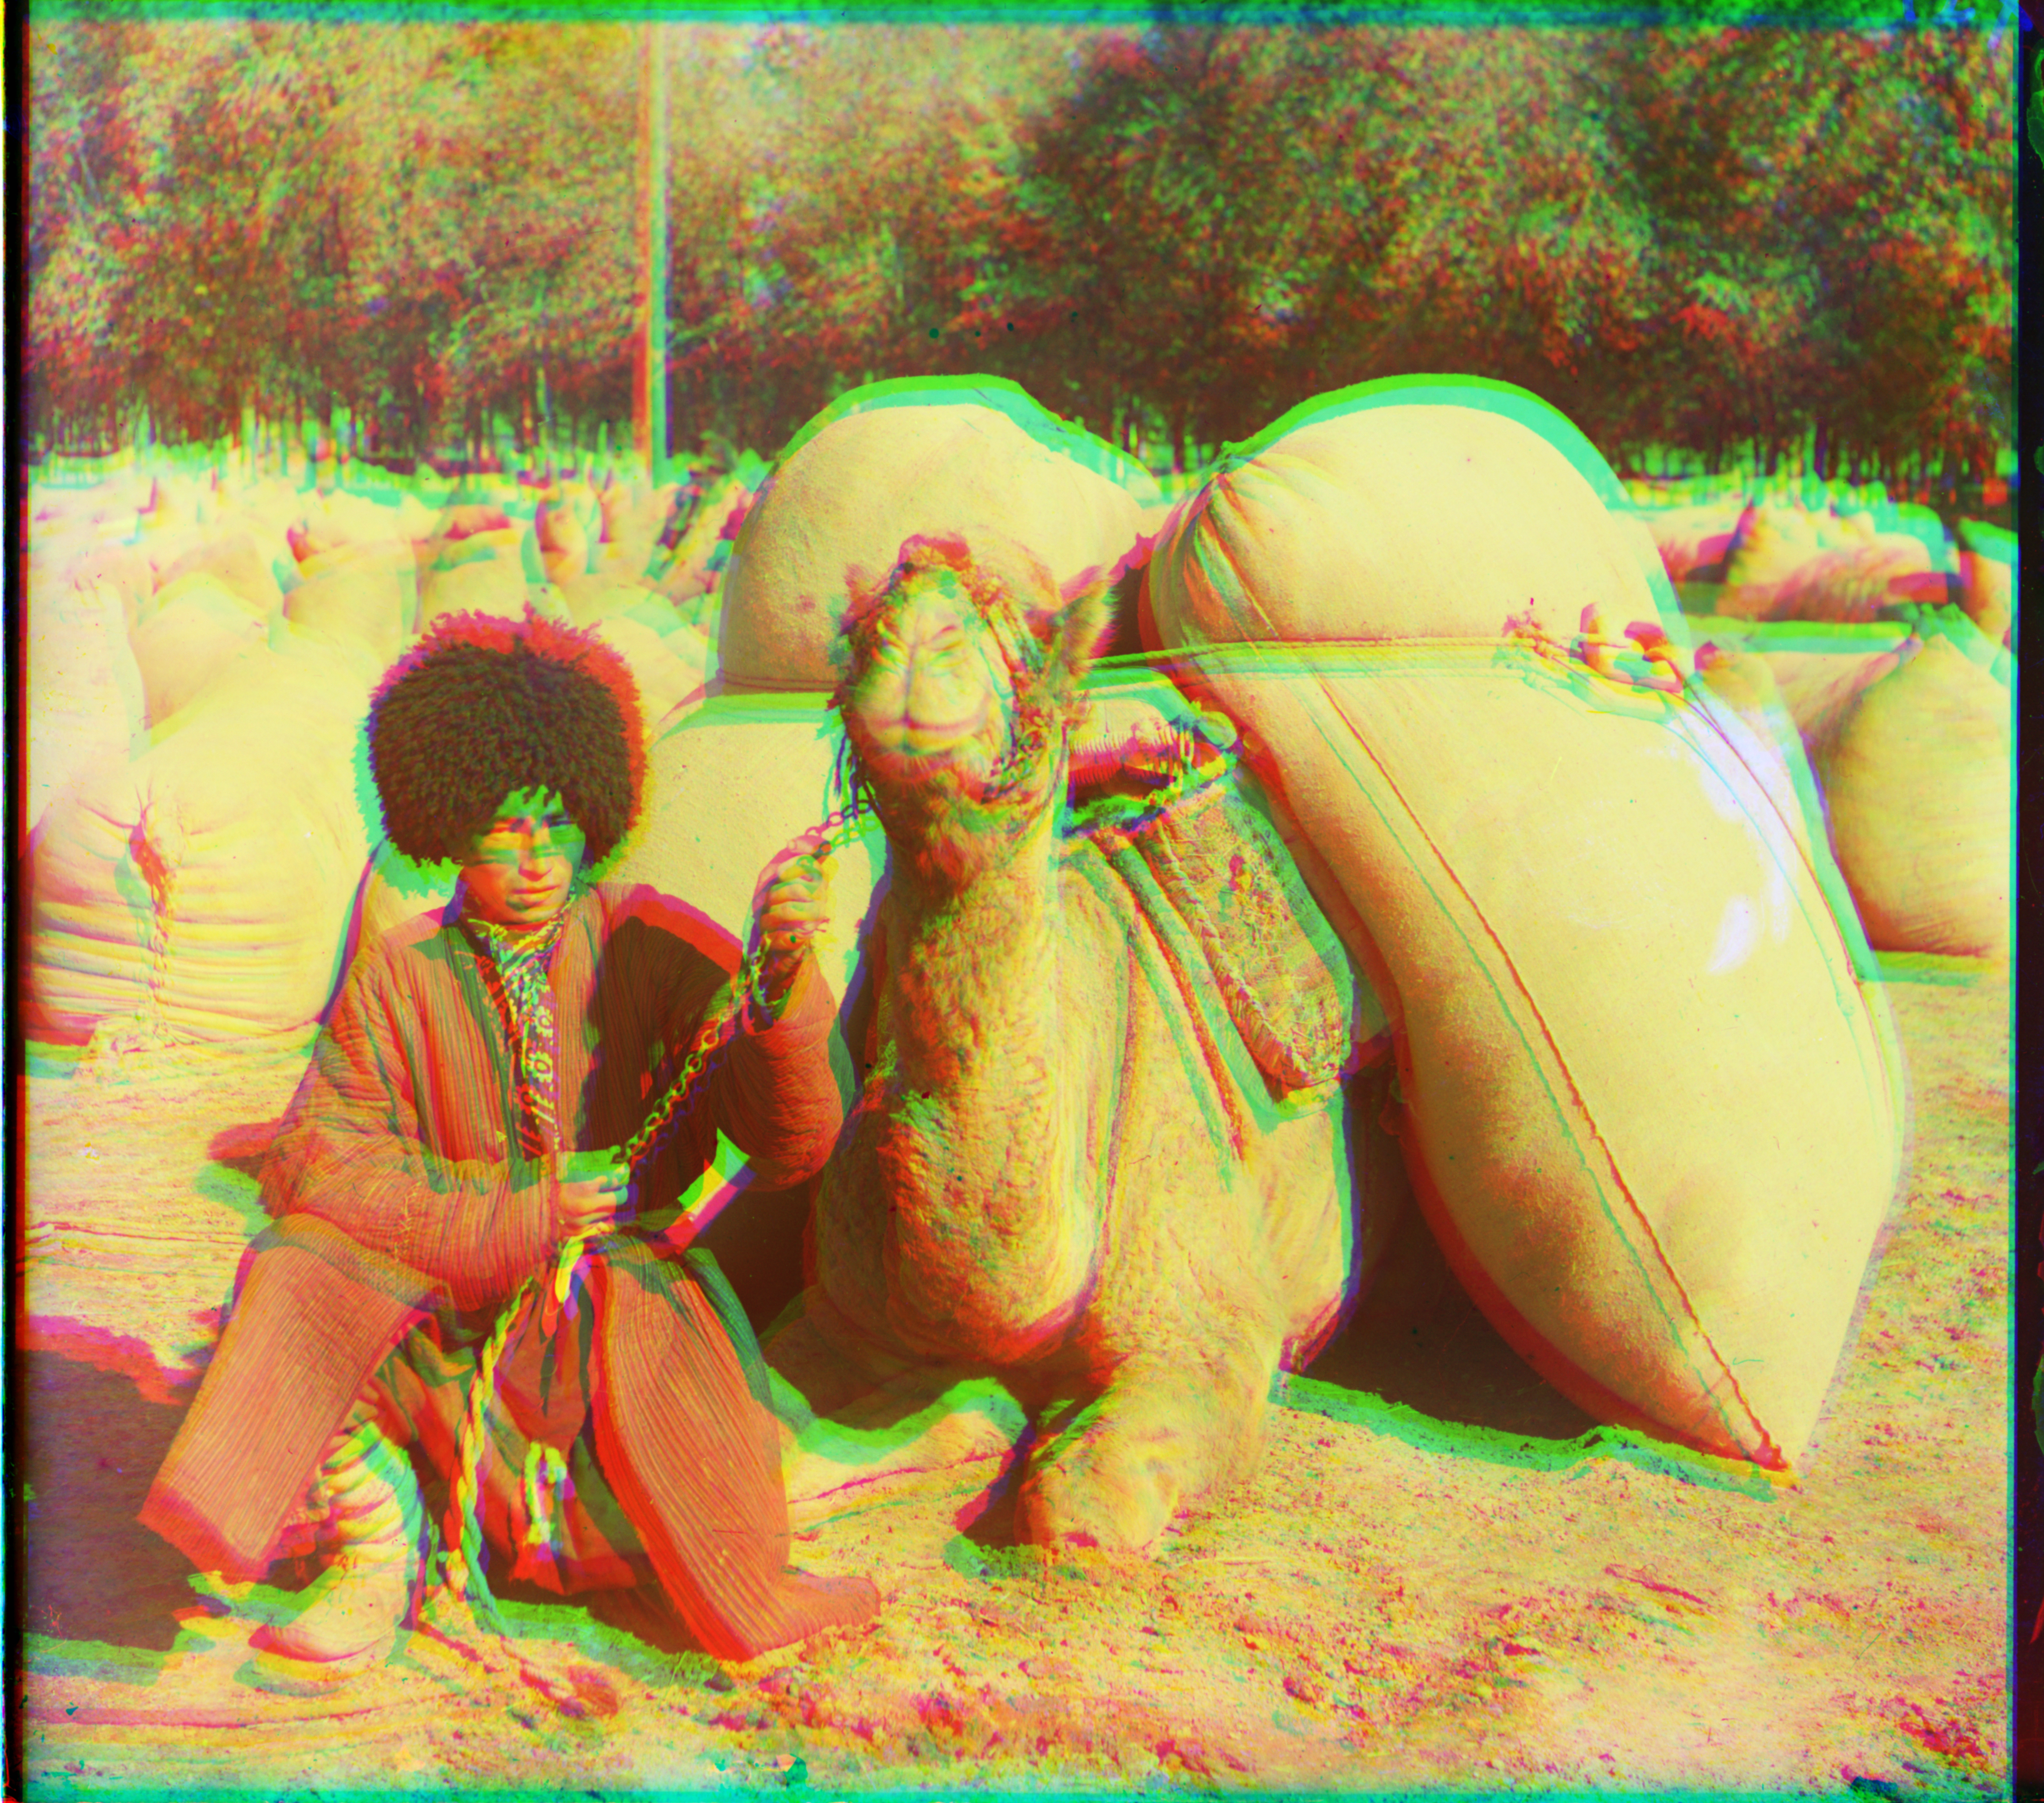
\includegraphics[scale=0.07]{../00011a/original}
\end{figure}

\begin{figure}[!htb]
\caption{SURF Aligned Composite 00011a}
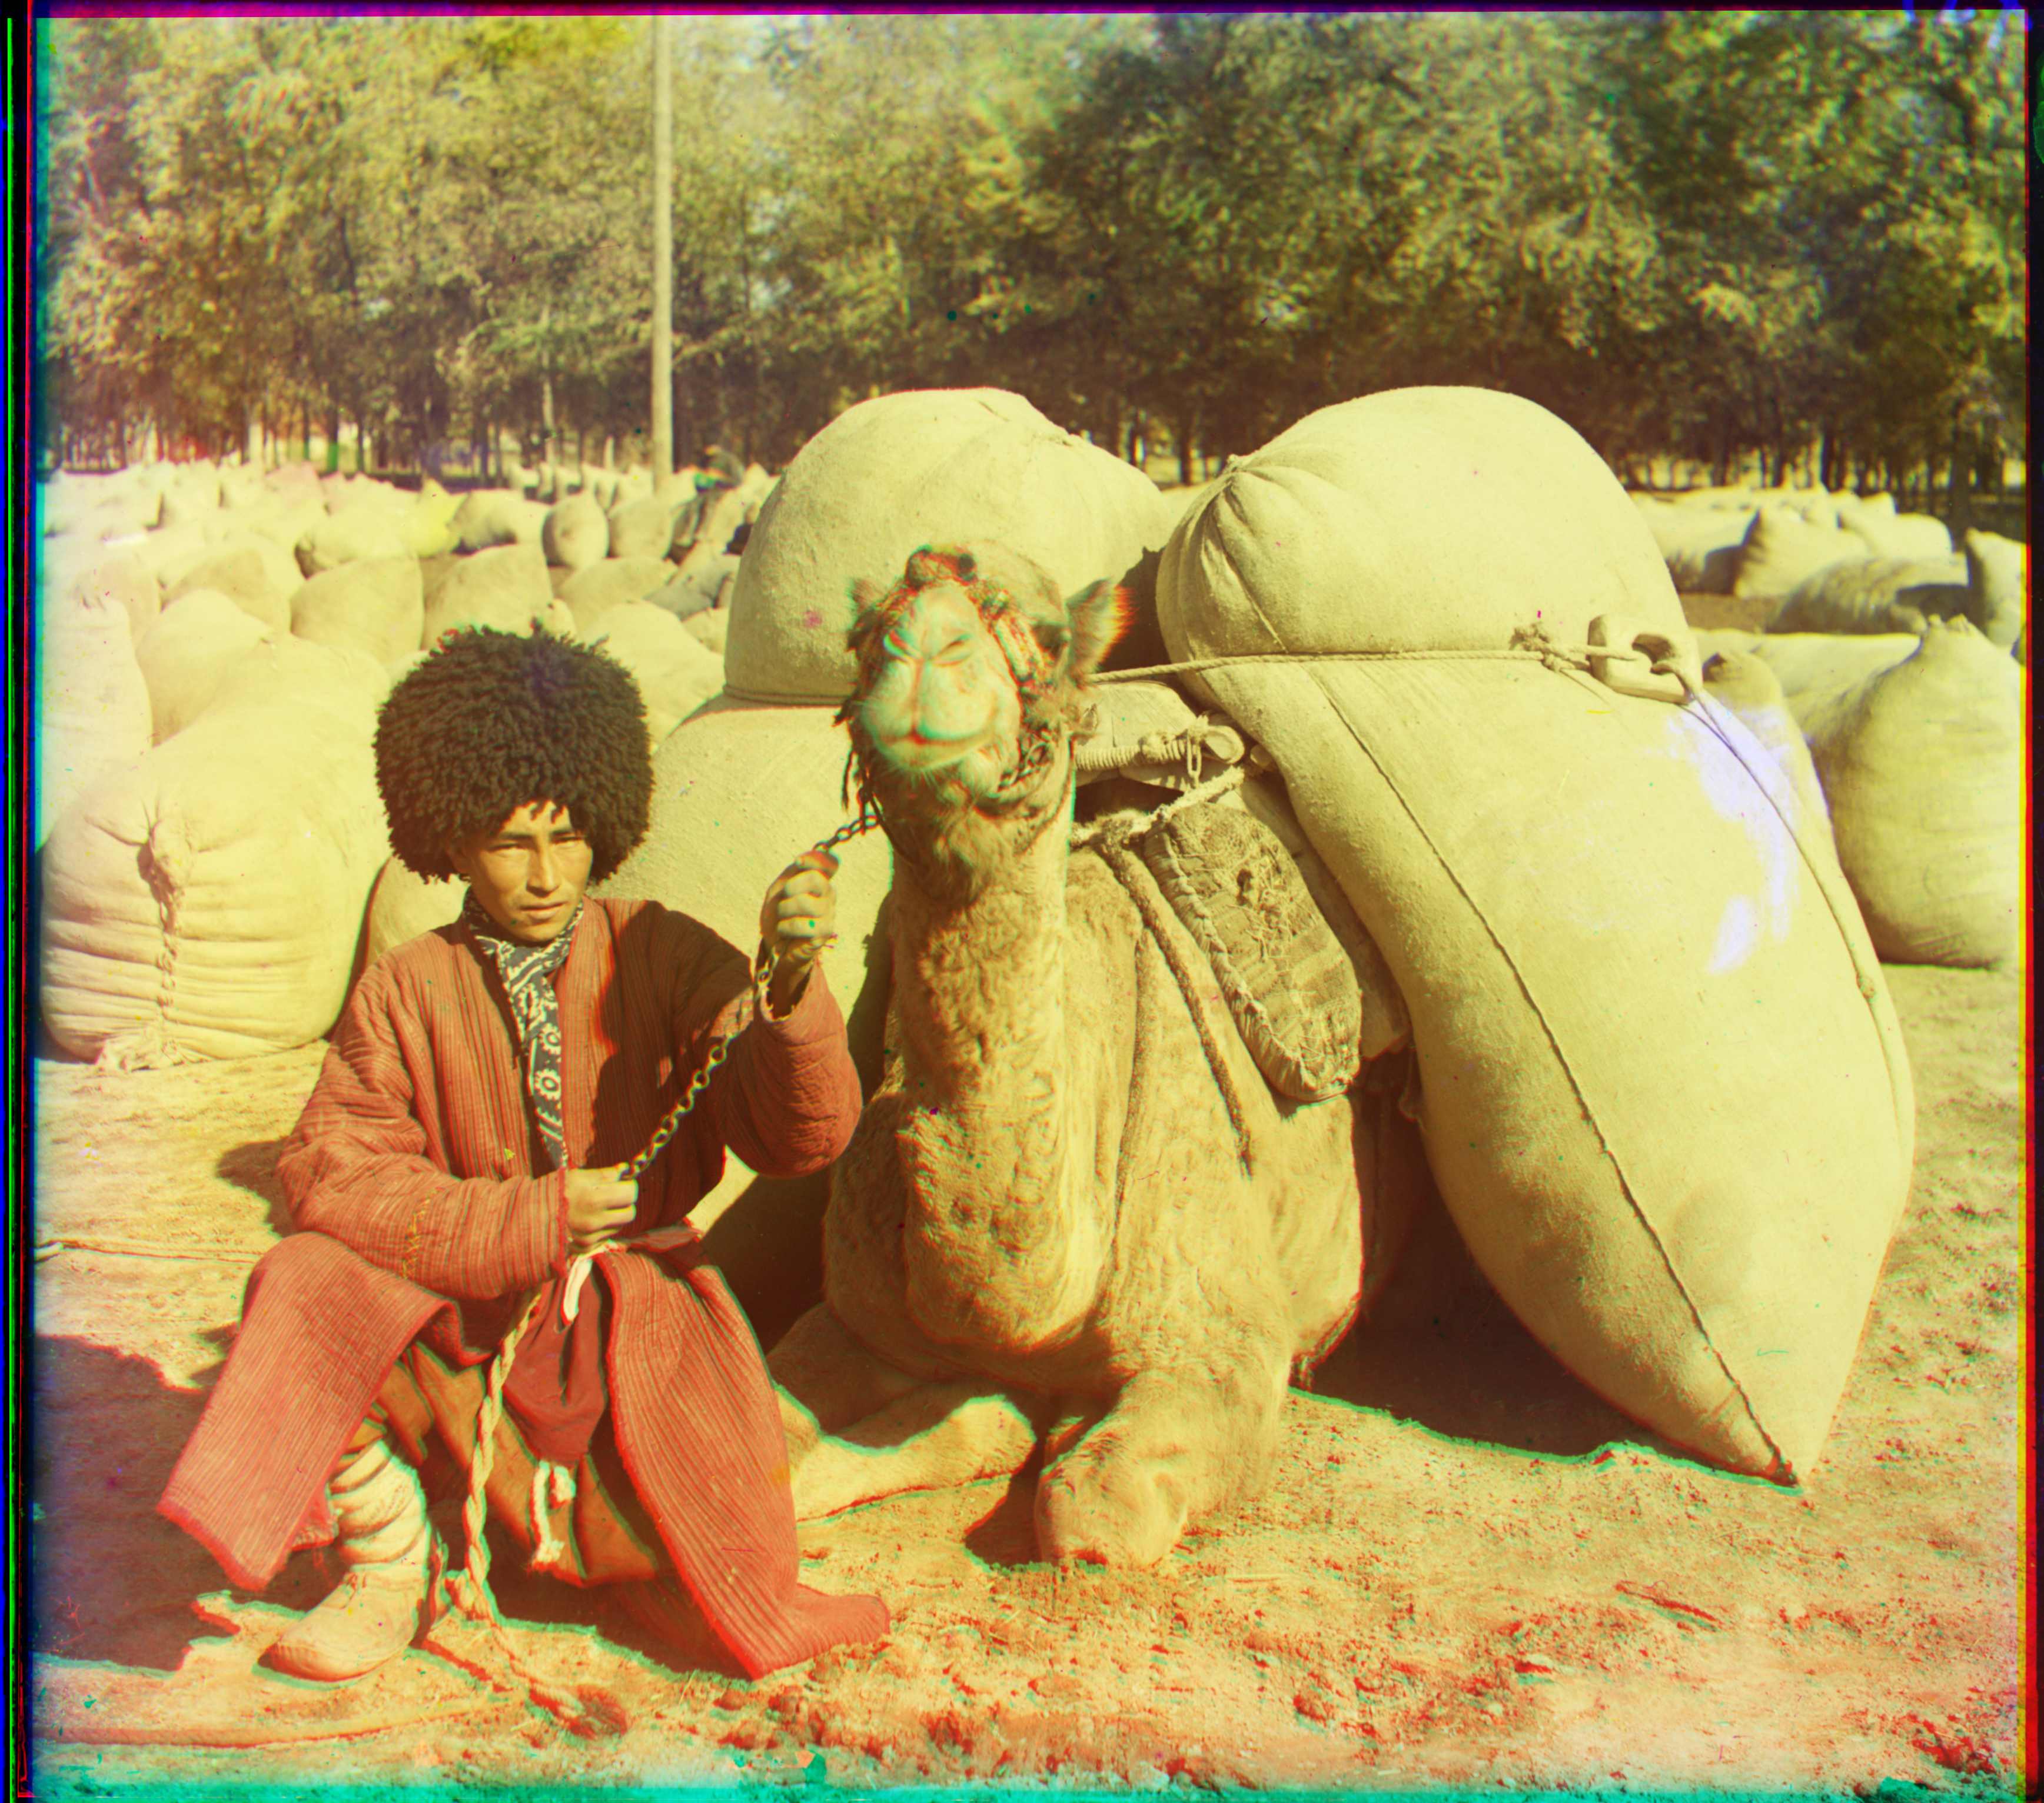
\includegraphics[scale=0.07]{../00011a/composite}
\end{figure}

\FloatBarrier

This is a picuter of presumably the same camel and now its owner. Same green ghosting along bottom lines and the same green bar along the bottom of the alinged image. 


\begin{figure}[!htb]
\caption{Rough Composite 00031a}
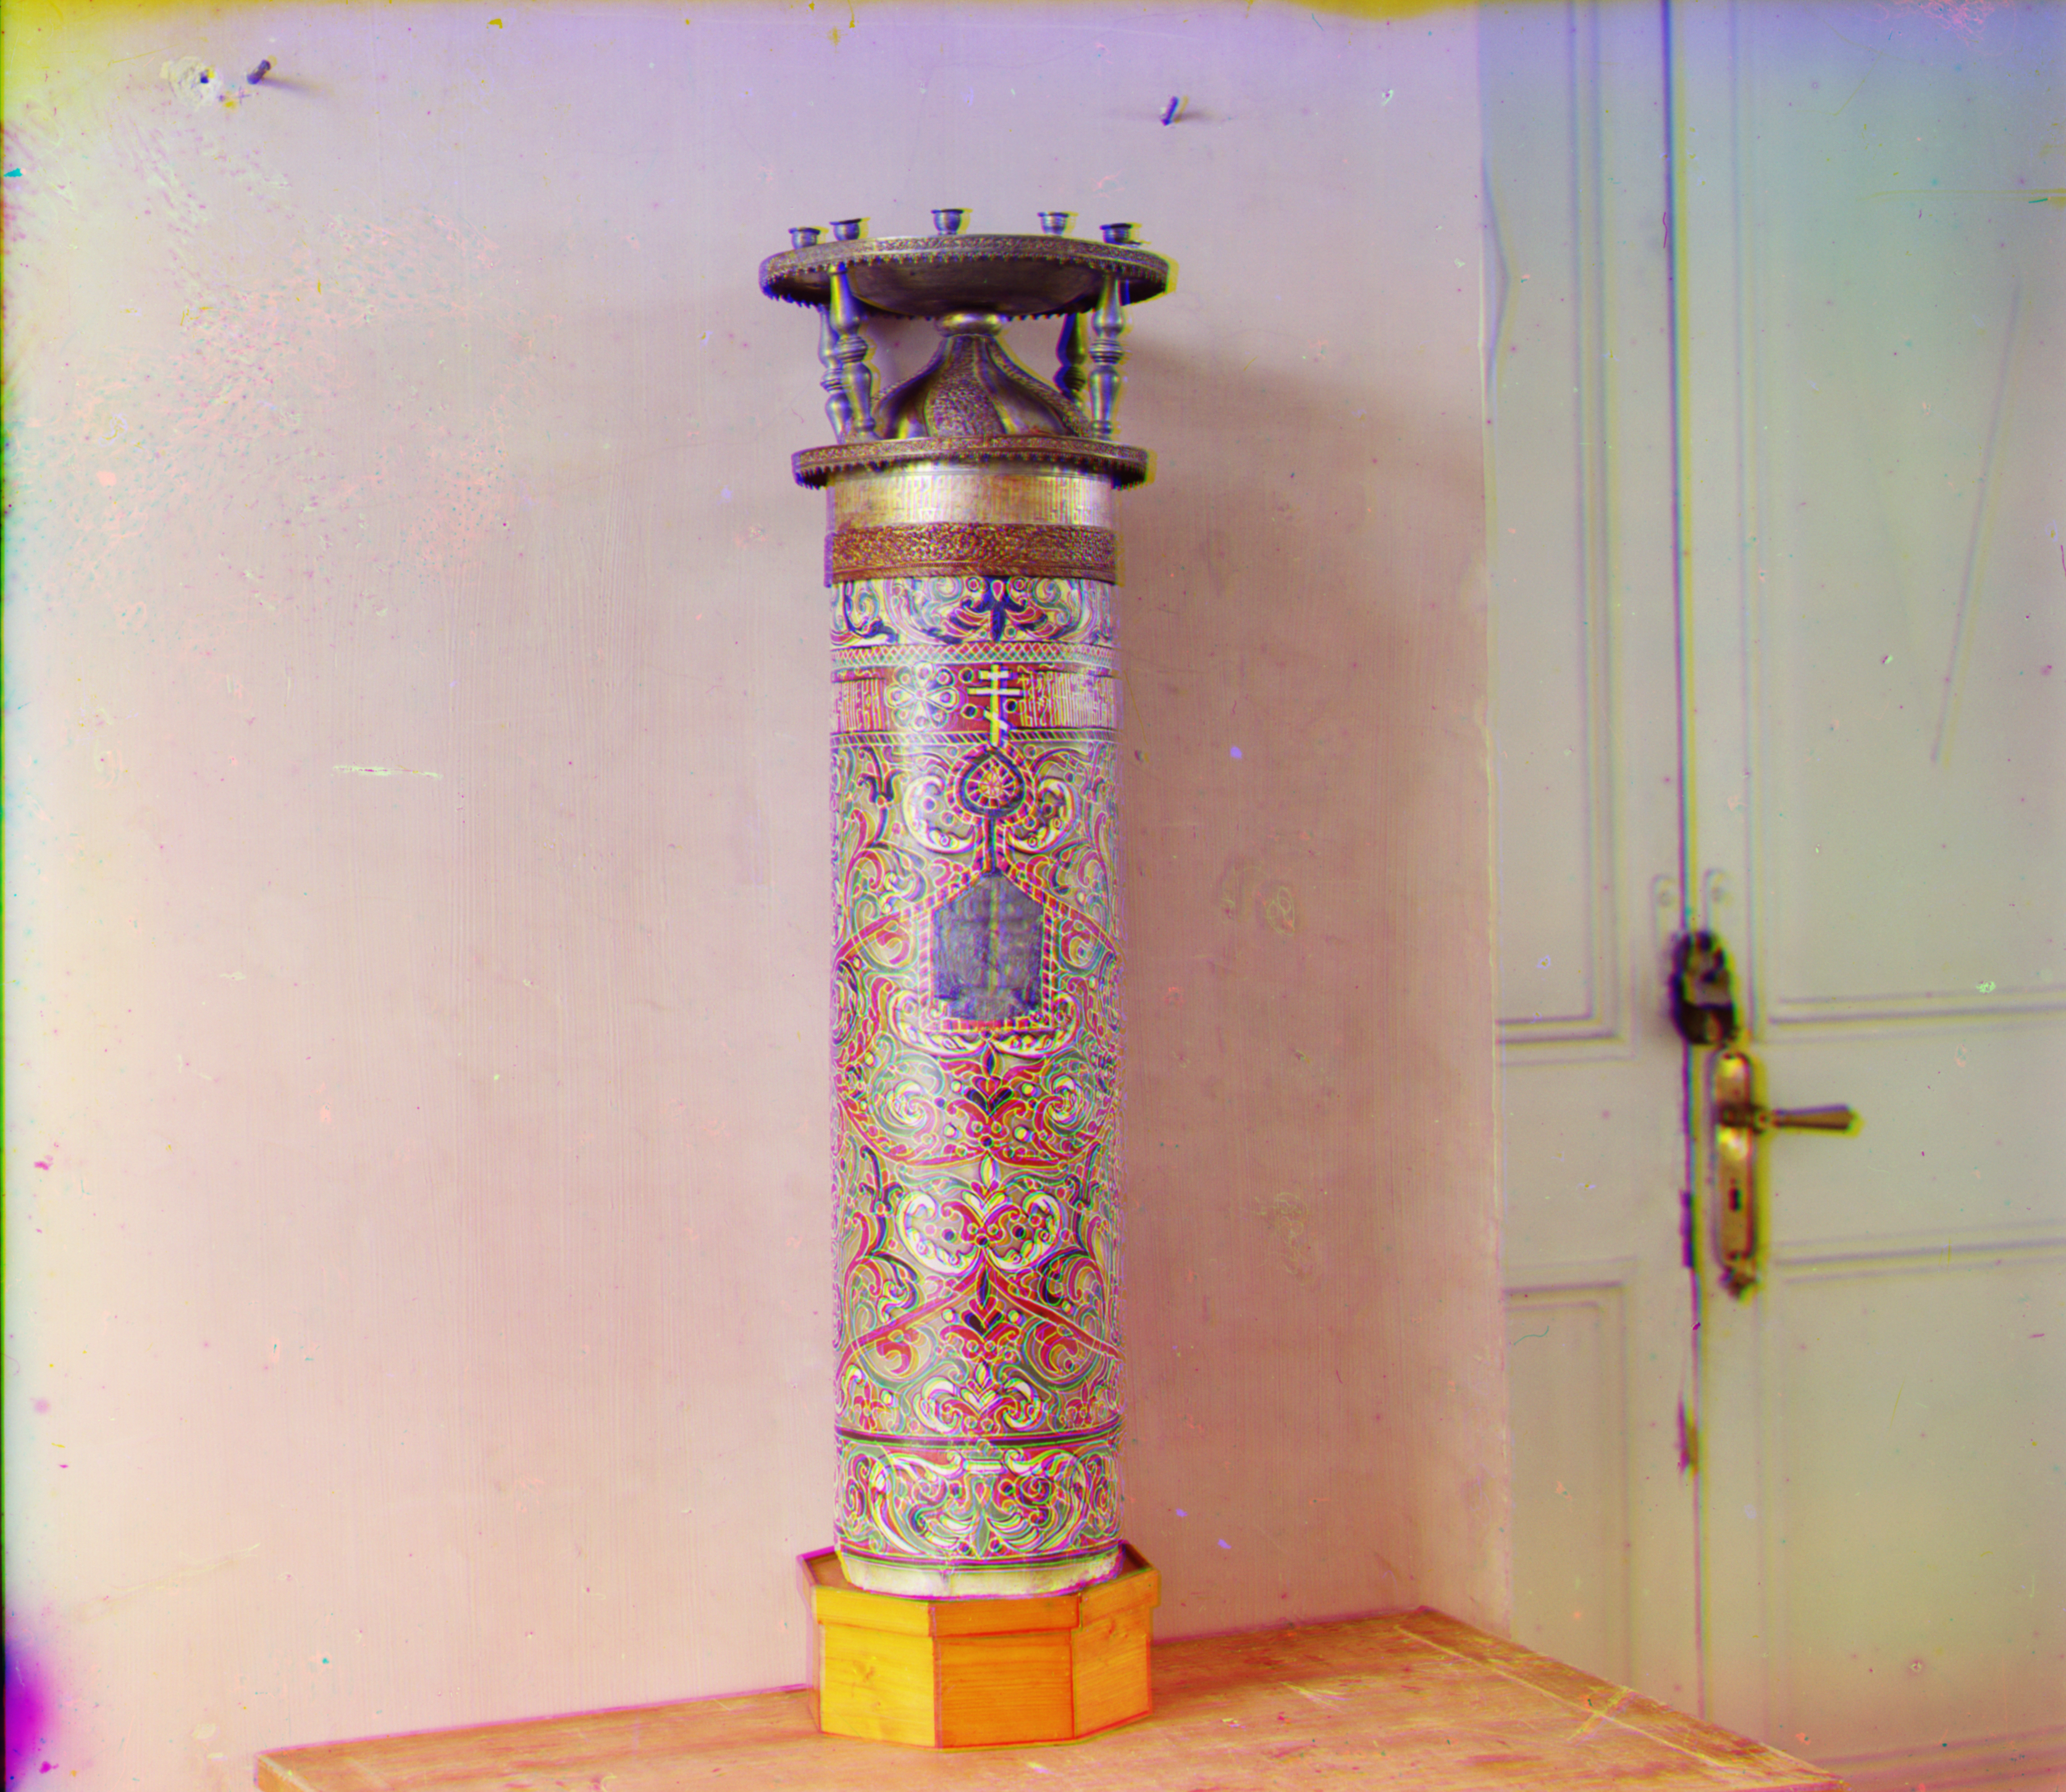
\includegraphics[scale=0.07]{../00031a/original}
\end{figure}

\begin{figure}[!htb]
\caption{SURF Aligned Composite 00031a}
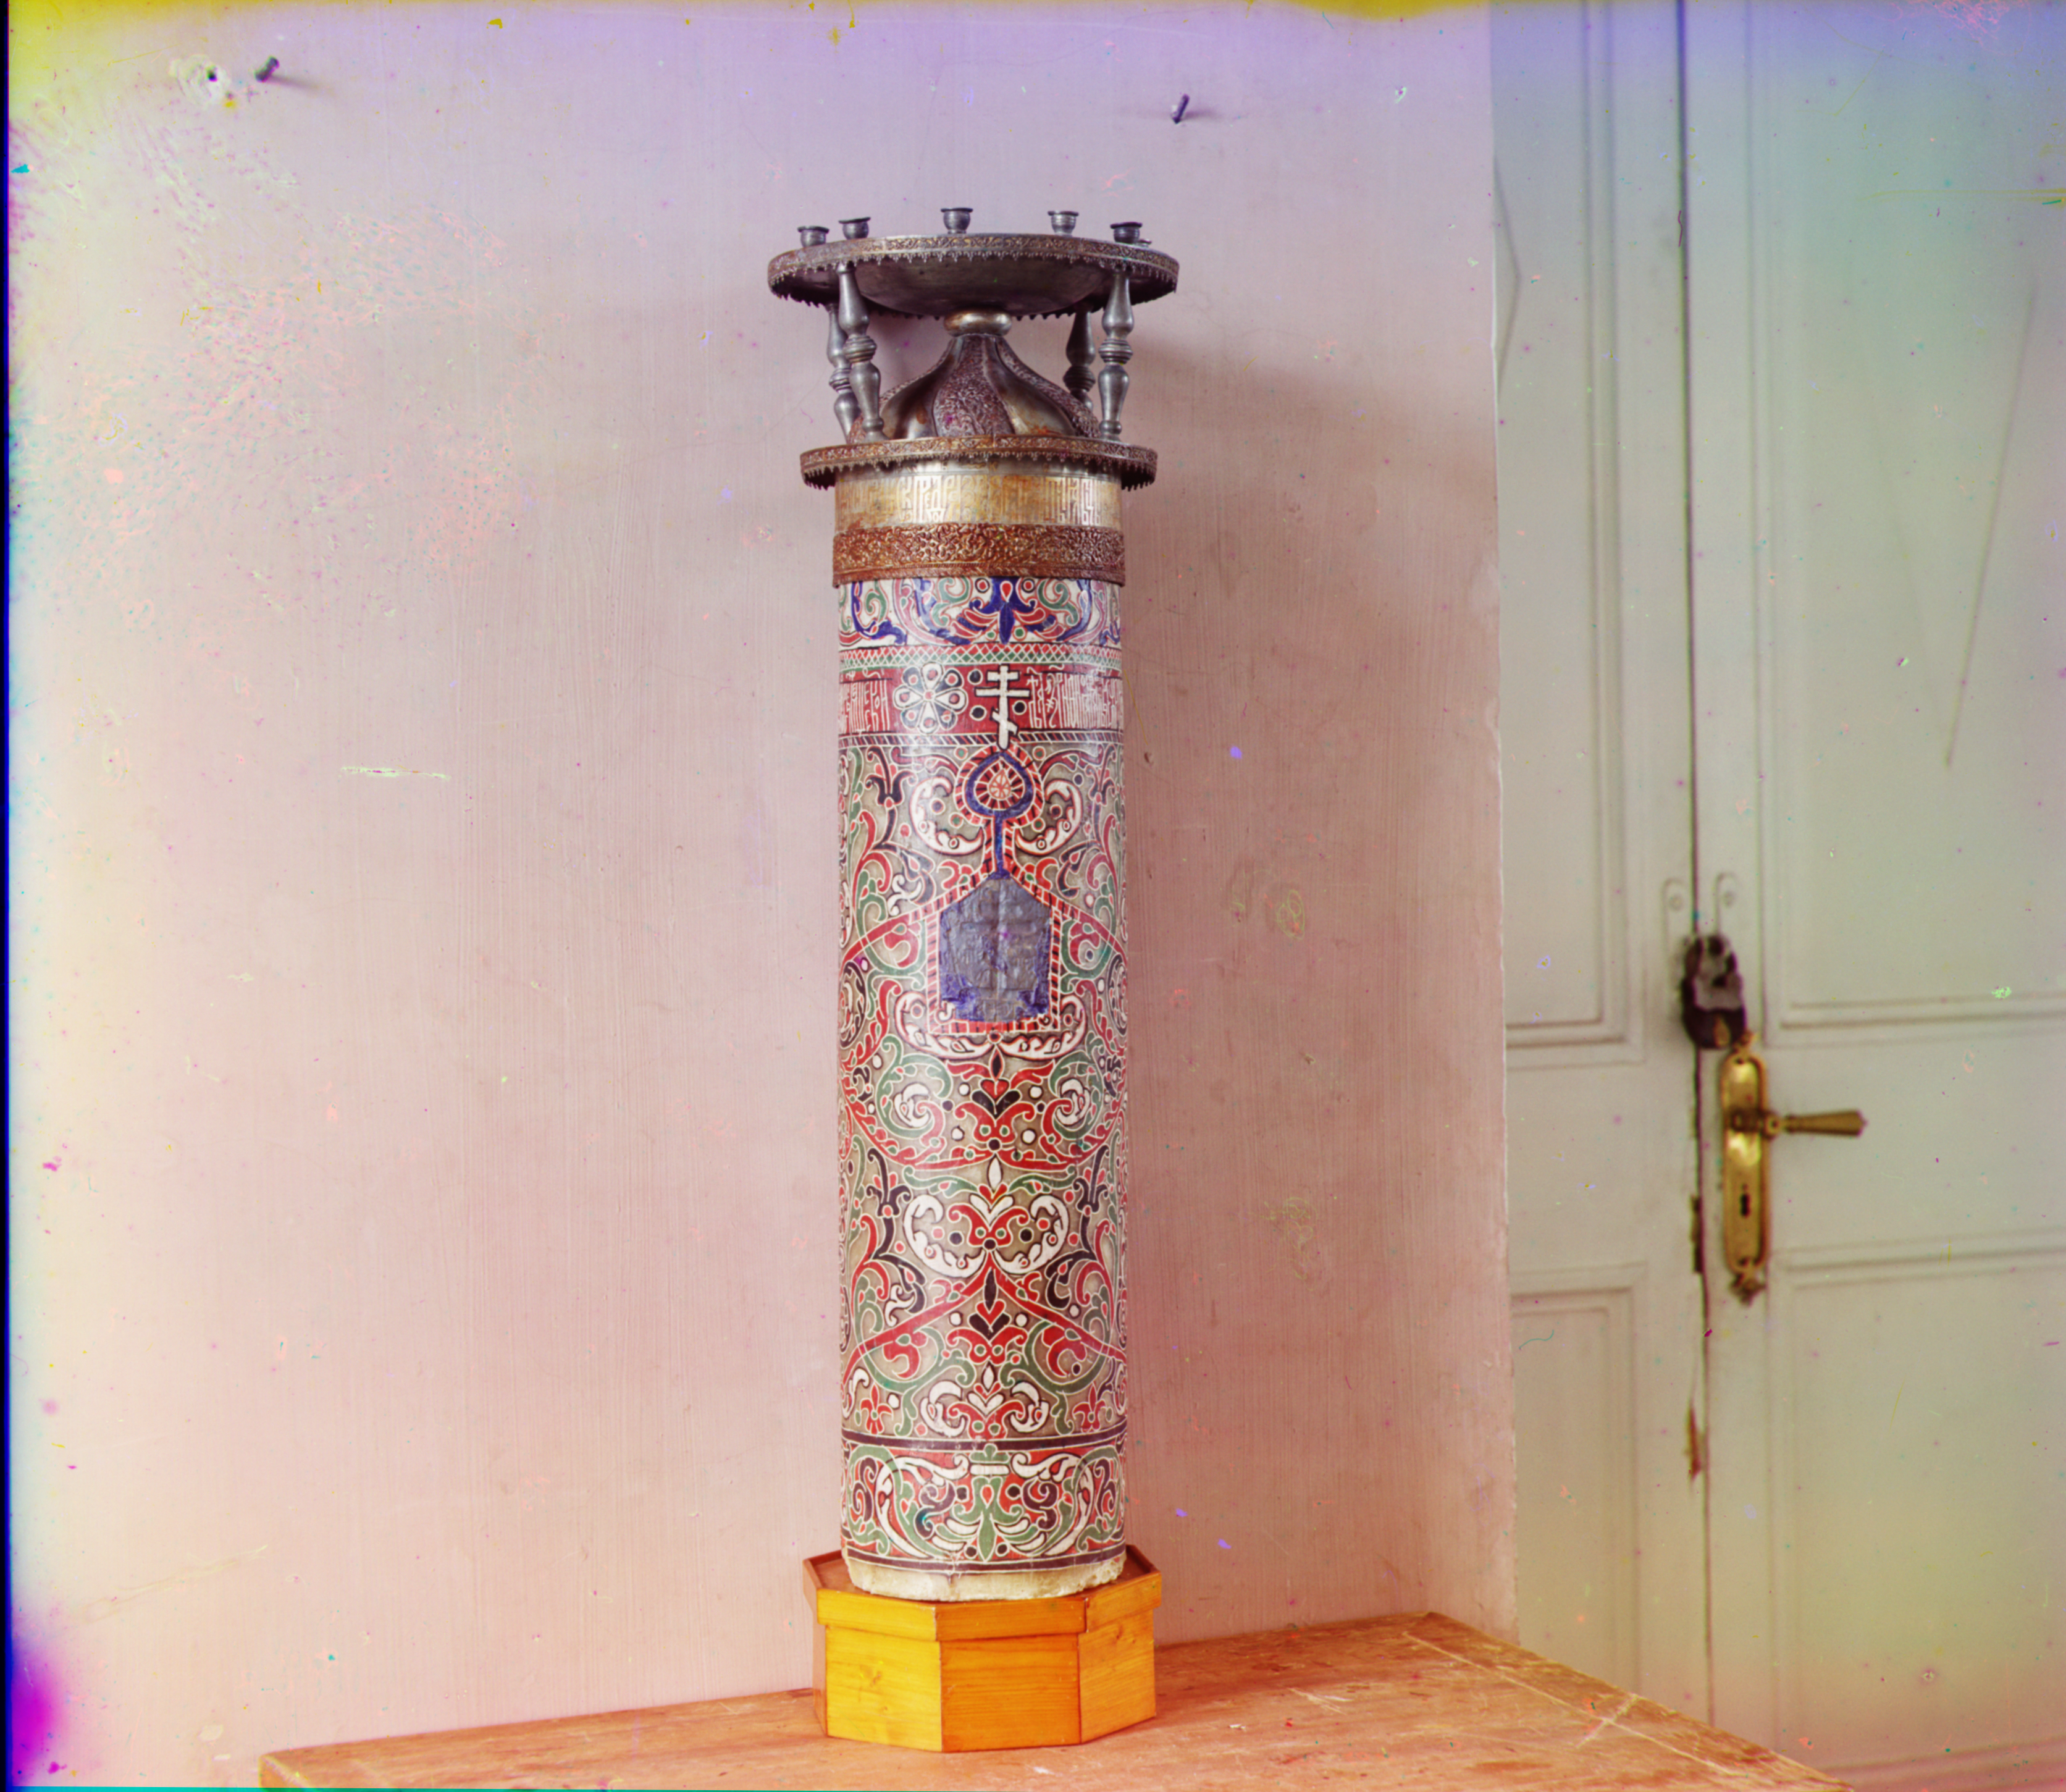
\includegraphics[scale=0.07]{../00031a/composite}
\end{figure}

\FloatBarrier

Rough composite looks decent, but there is some shift in the blue image a bit, noted by the yellow ghosting around right sides of the candle holder? and the door handle. This is eliminated in the aligned image. 

\begin{figure}[!htb]
\caption{Rough Composite 00111a}
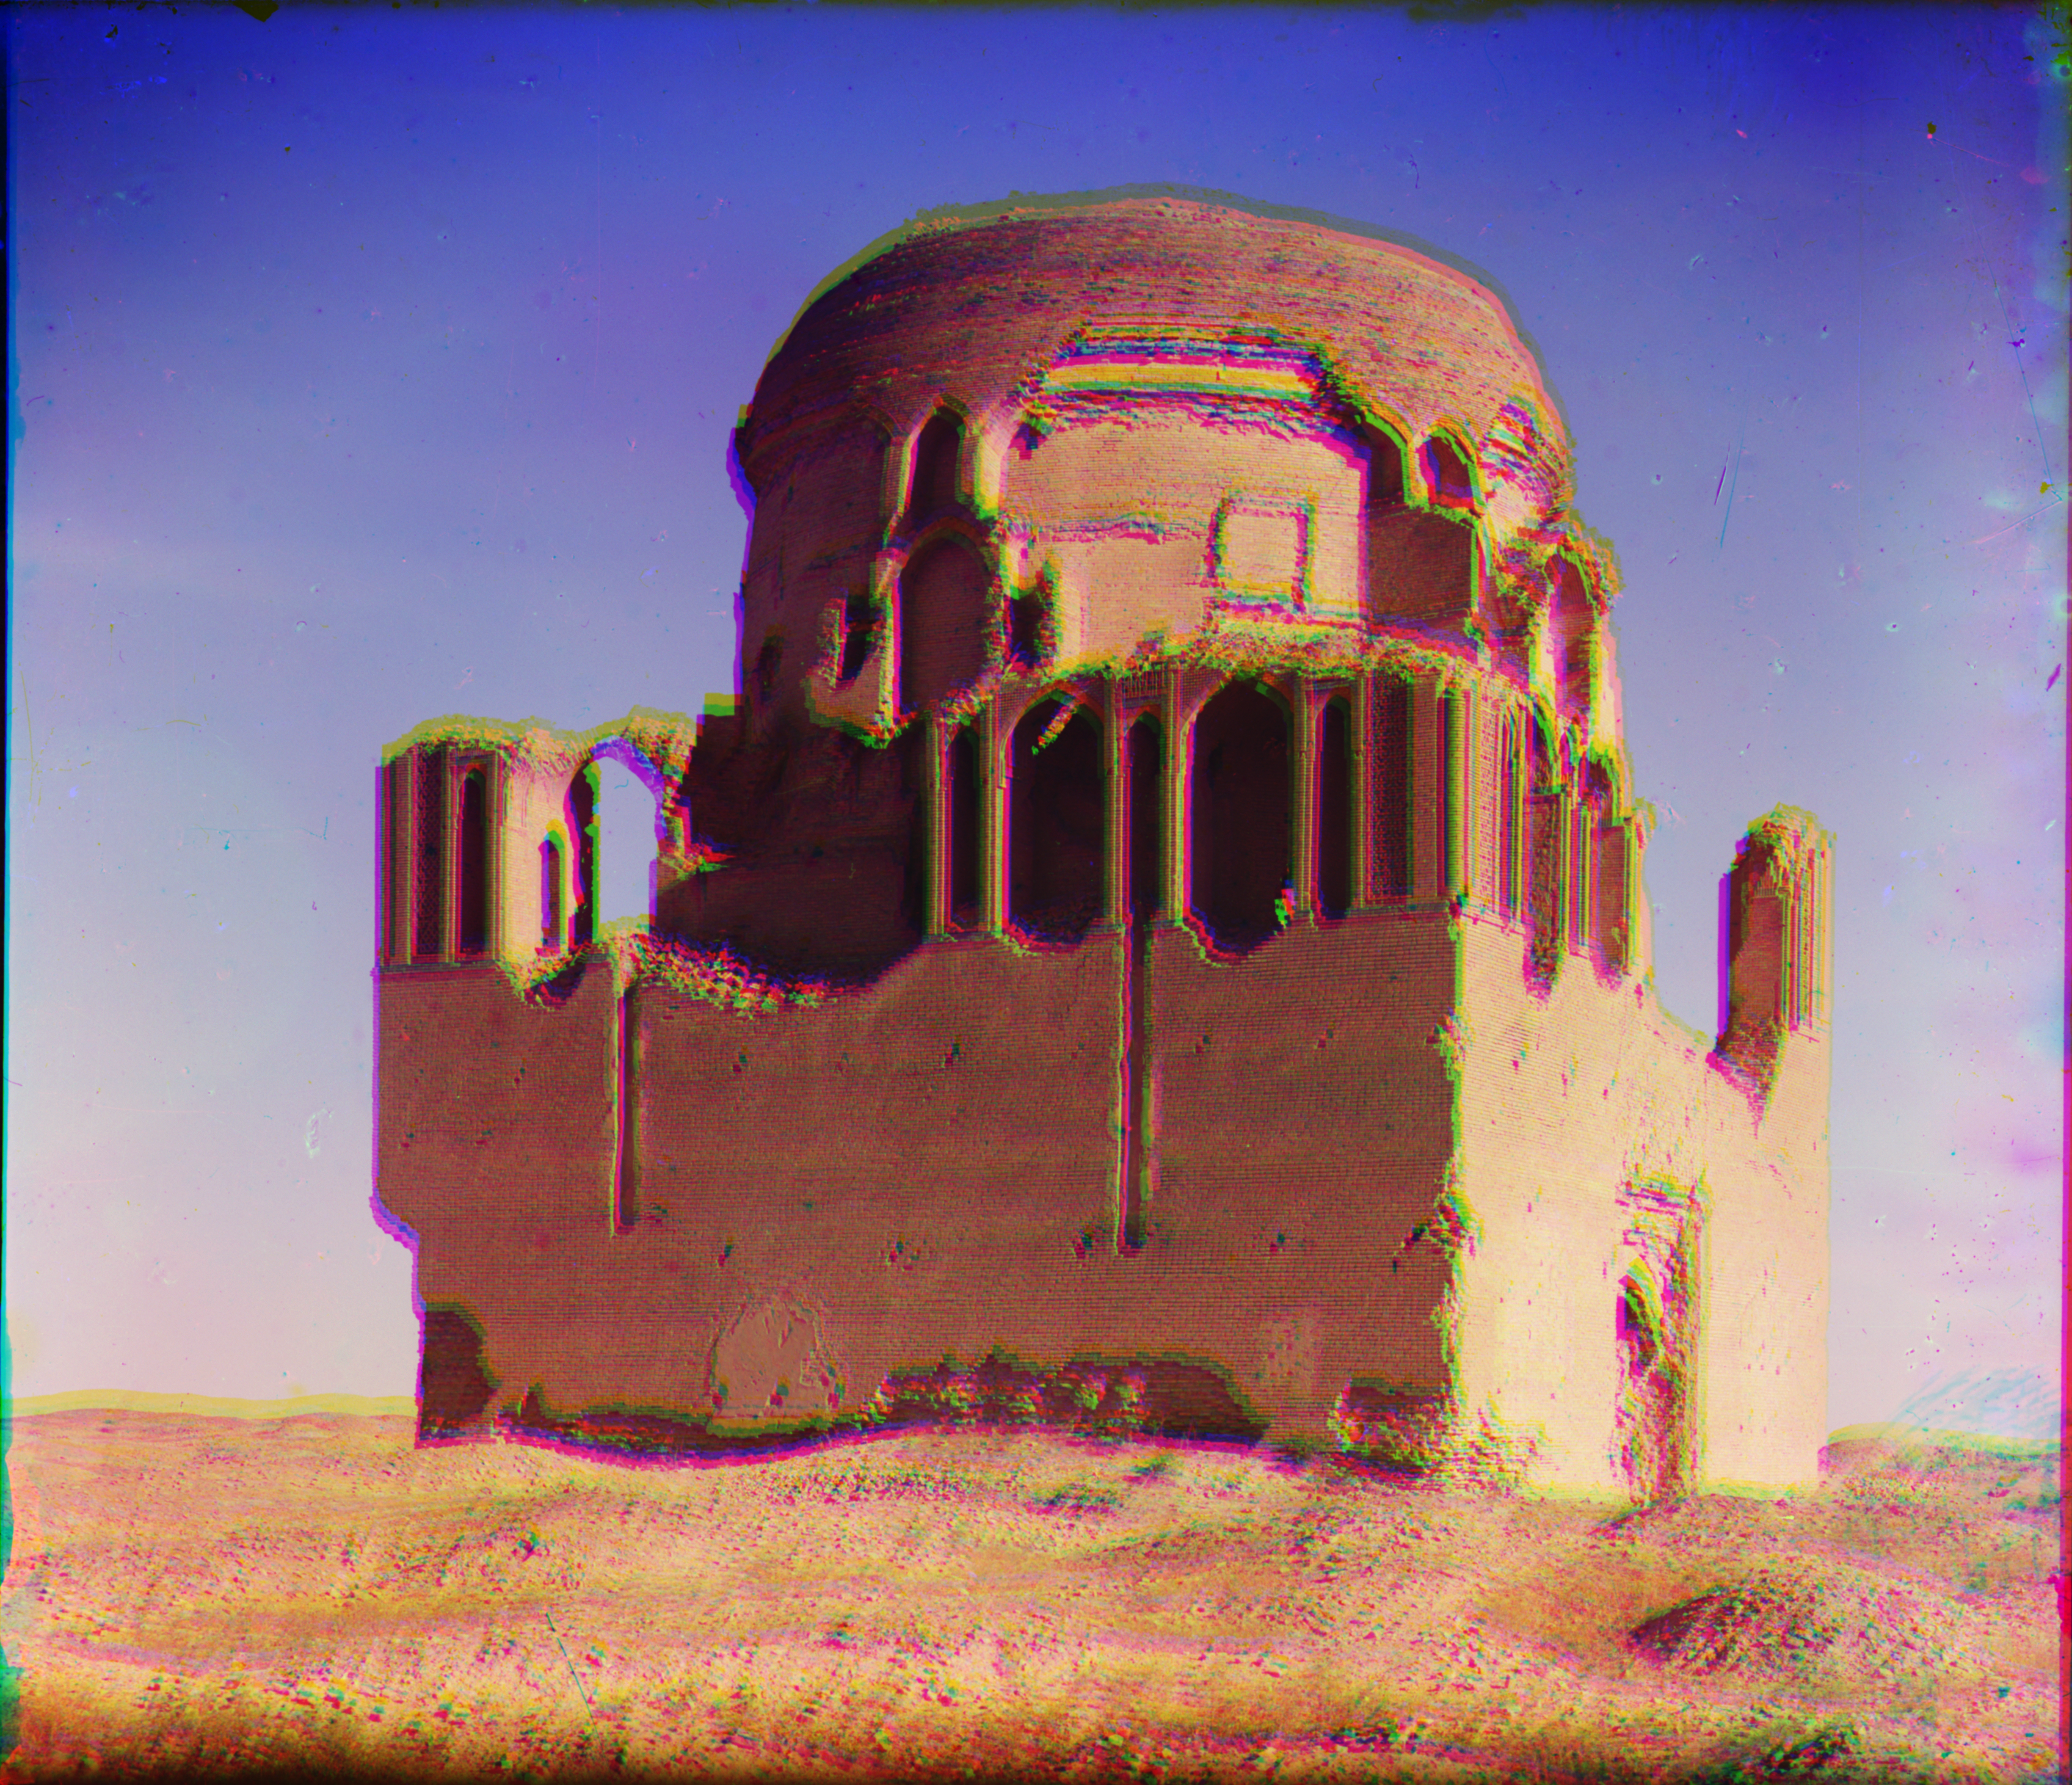
\includegraphics[scale=0.07]{../00111a/original}
\end{figure}

\begin{figure}[!htb]
\caption{SURF Aligned Composite 00111a}
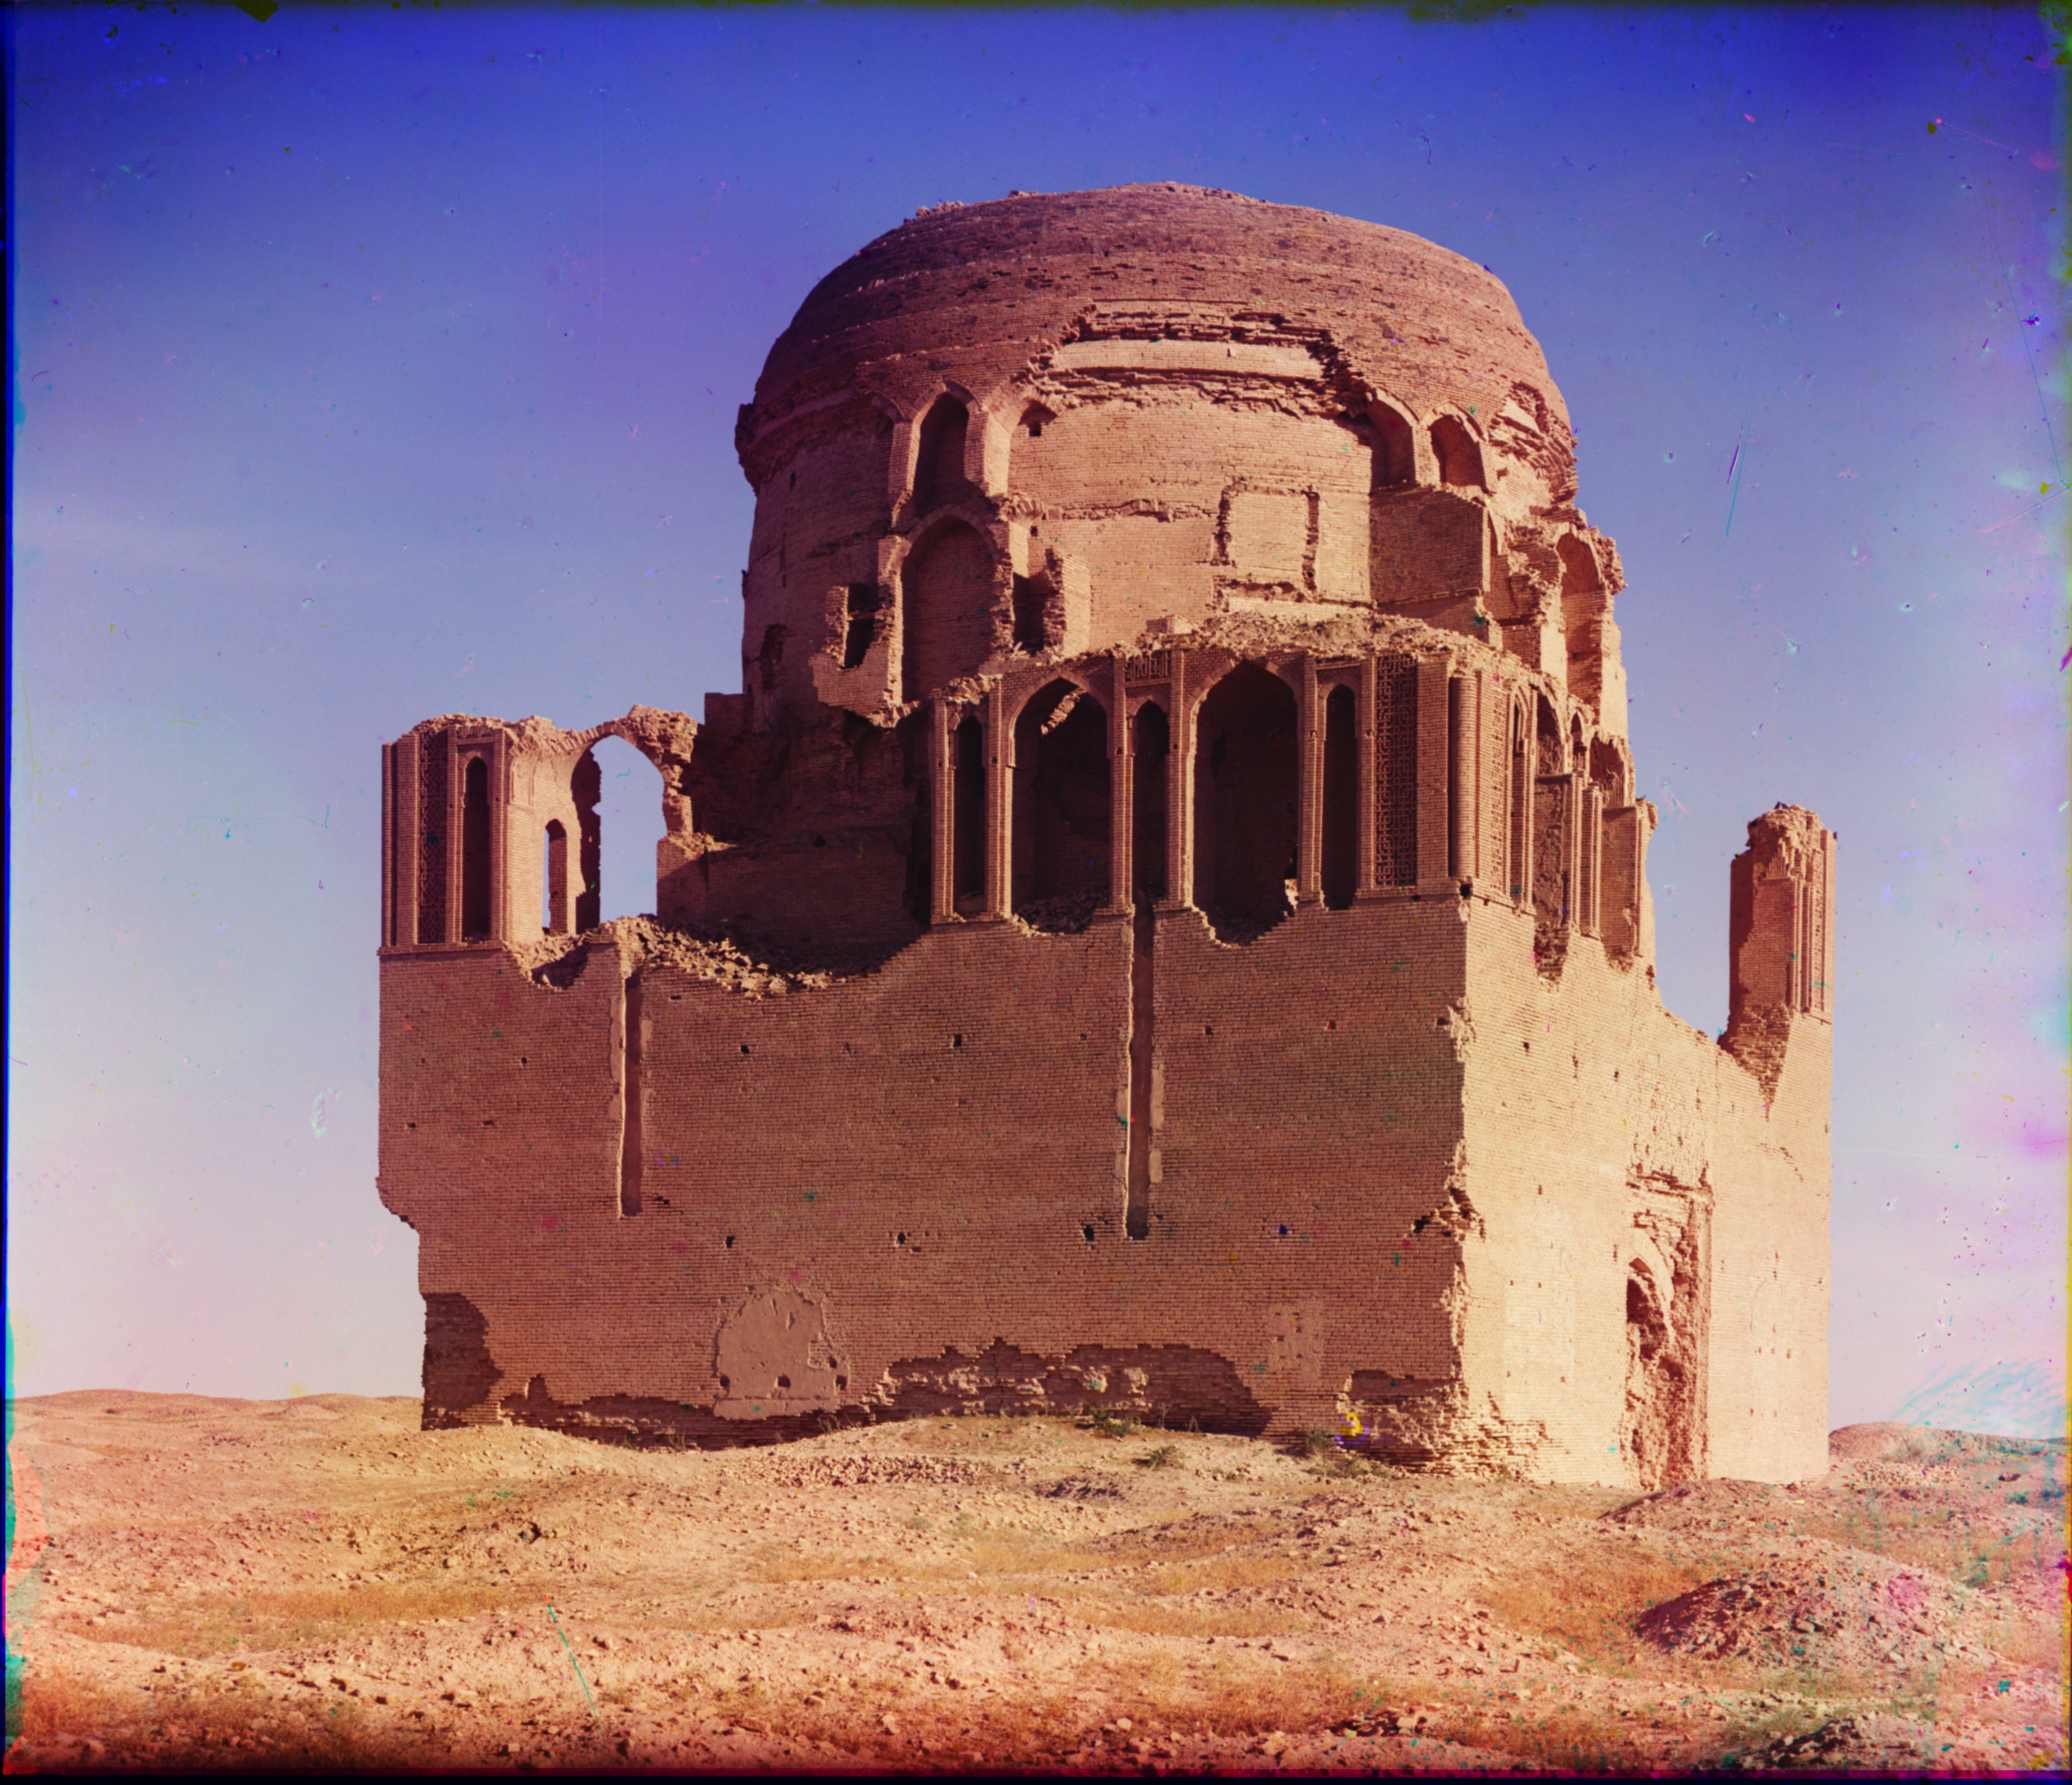
\includegraphics[scale=0.07]{../00111a/composite}
\end{figure}

\FloatBarrier

Blue image is shifted downwards, causing some blue outline along the bottom and yellow outline along the top of the ruins's features. There is also some green along the yellow outlines and purple near the bottom as the red image is very off centre. These are elimated in the aligned image, save for a few coloured splotches cause by different capture atrifacts in each image. 


\begin{figure}[!htb]
\caption{Rough Composite 00152a}
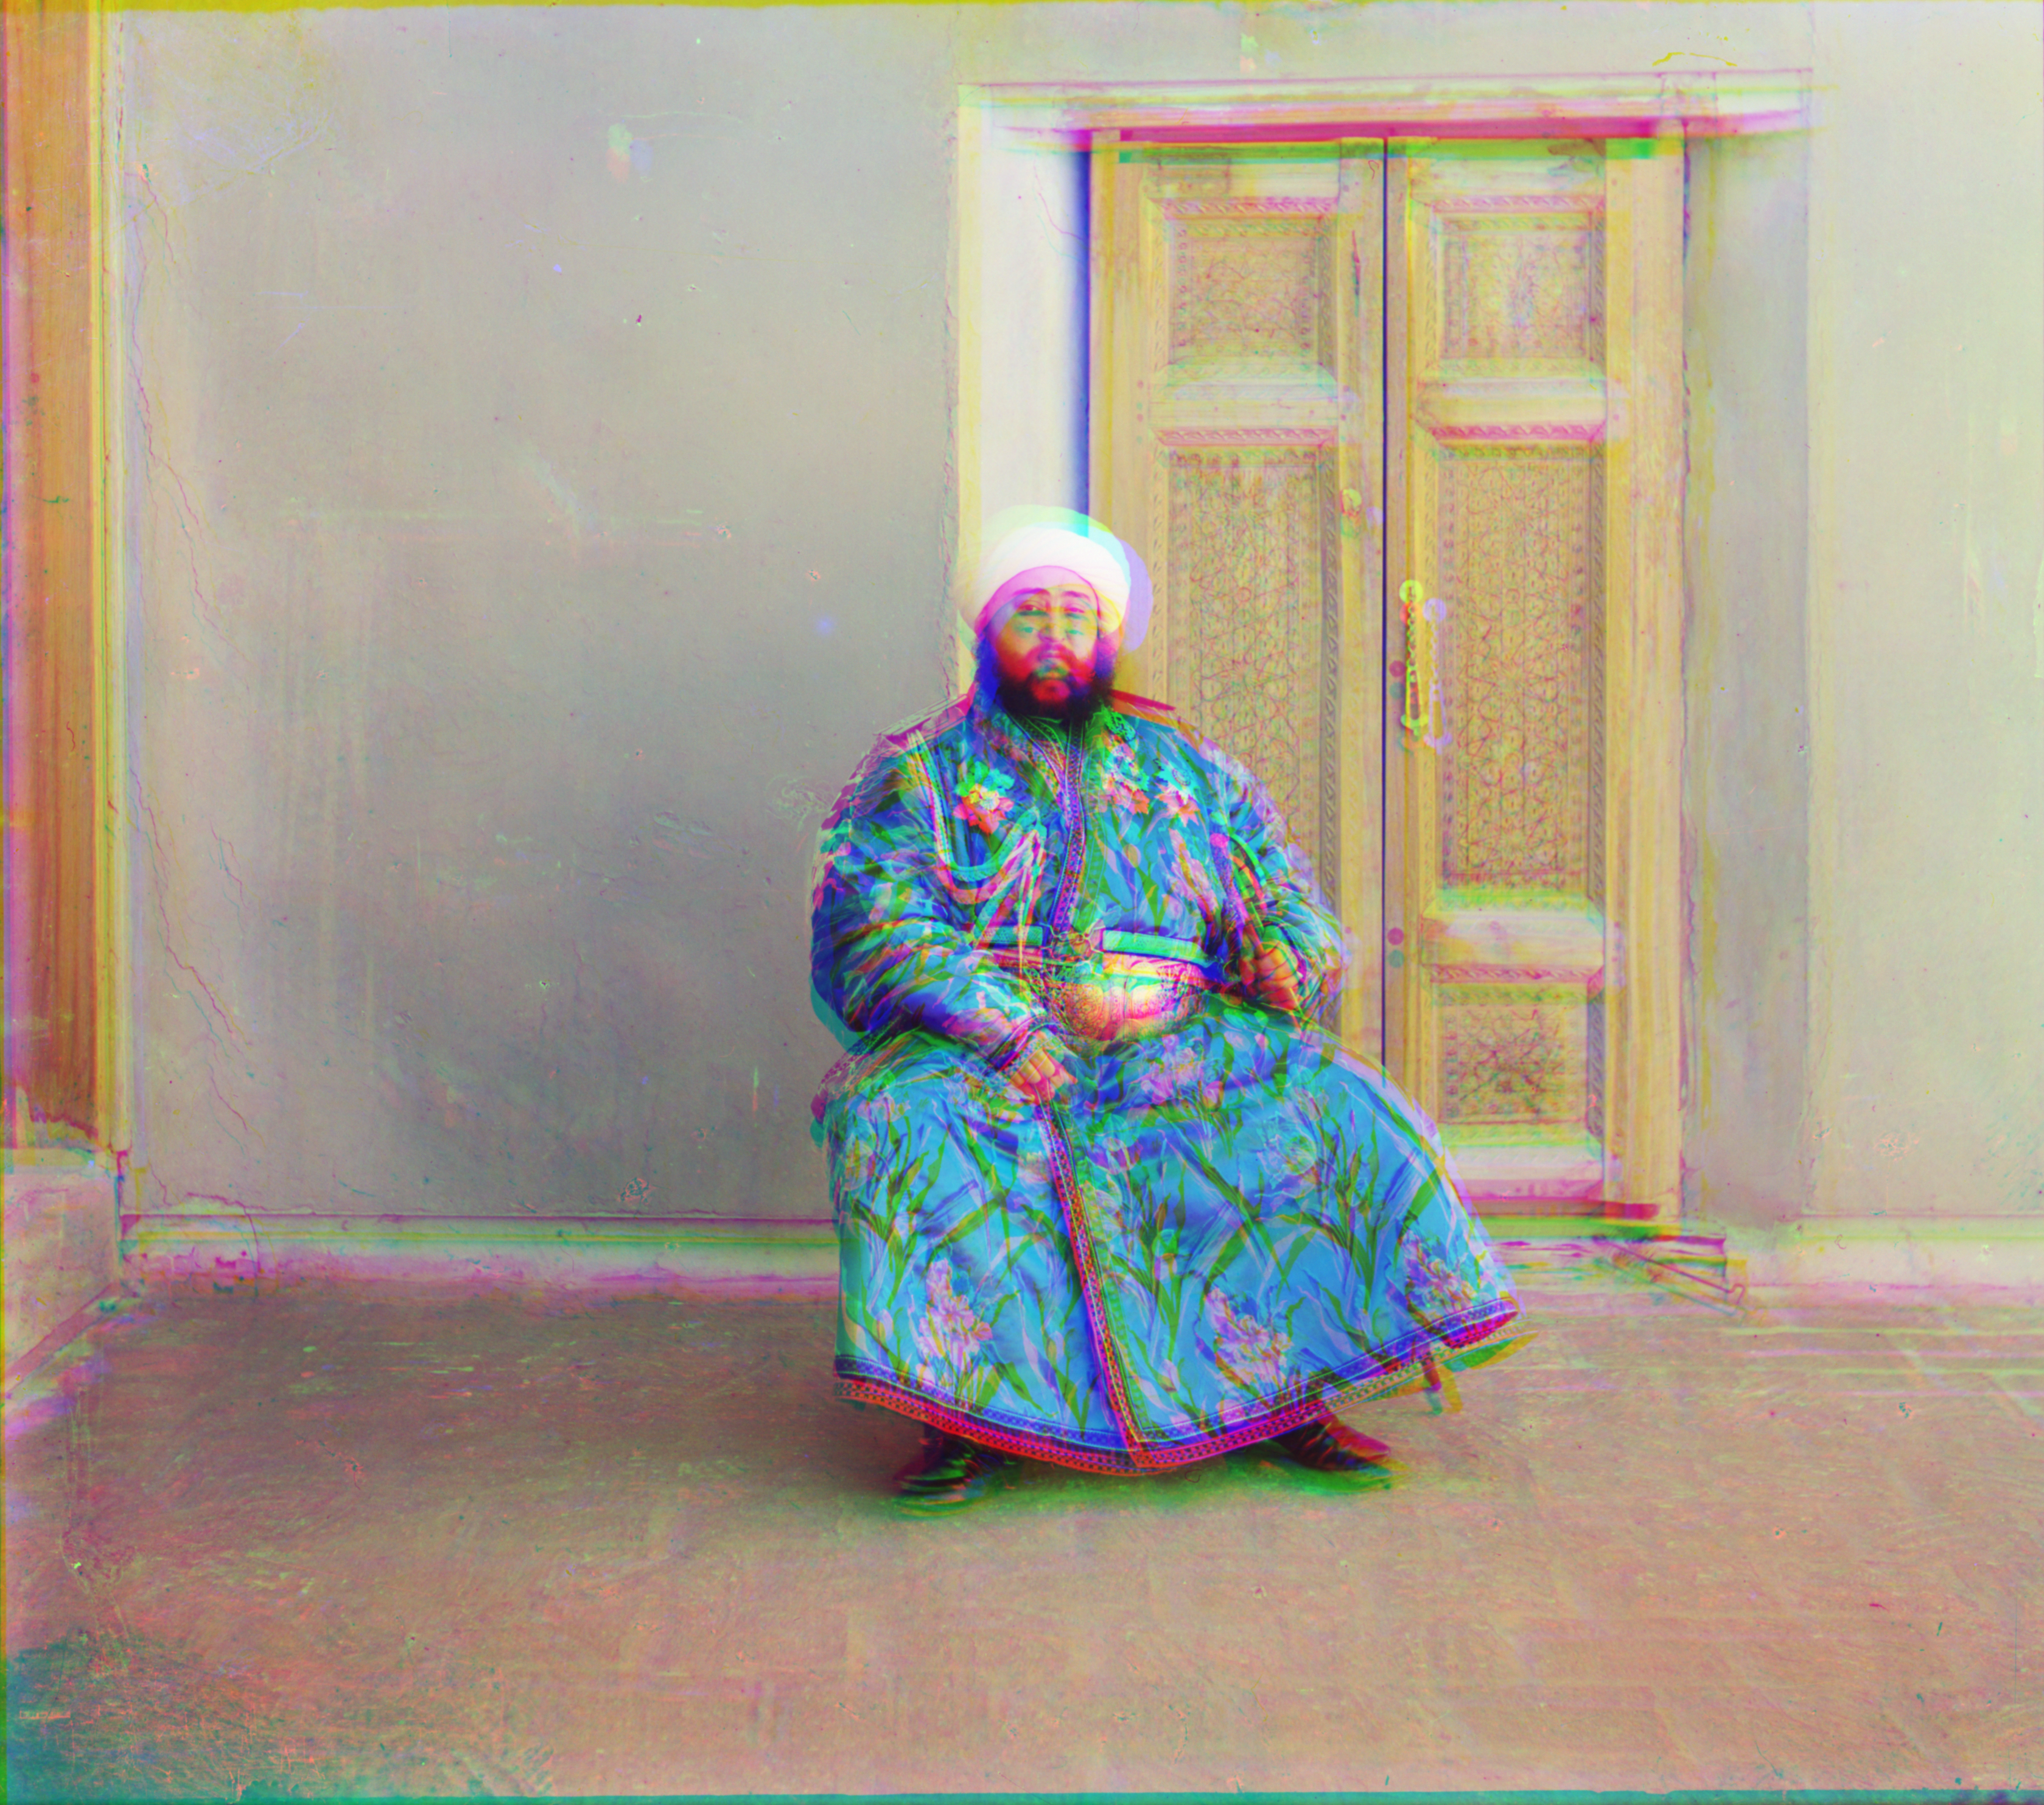
\includegraphics[scale=0.07]{../00152a/original}
\end{figure}

\begin{figure}[!htb]
\caption{SURF Aligned Composite 00152a}
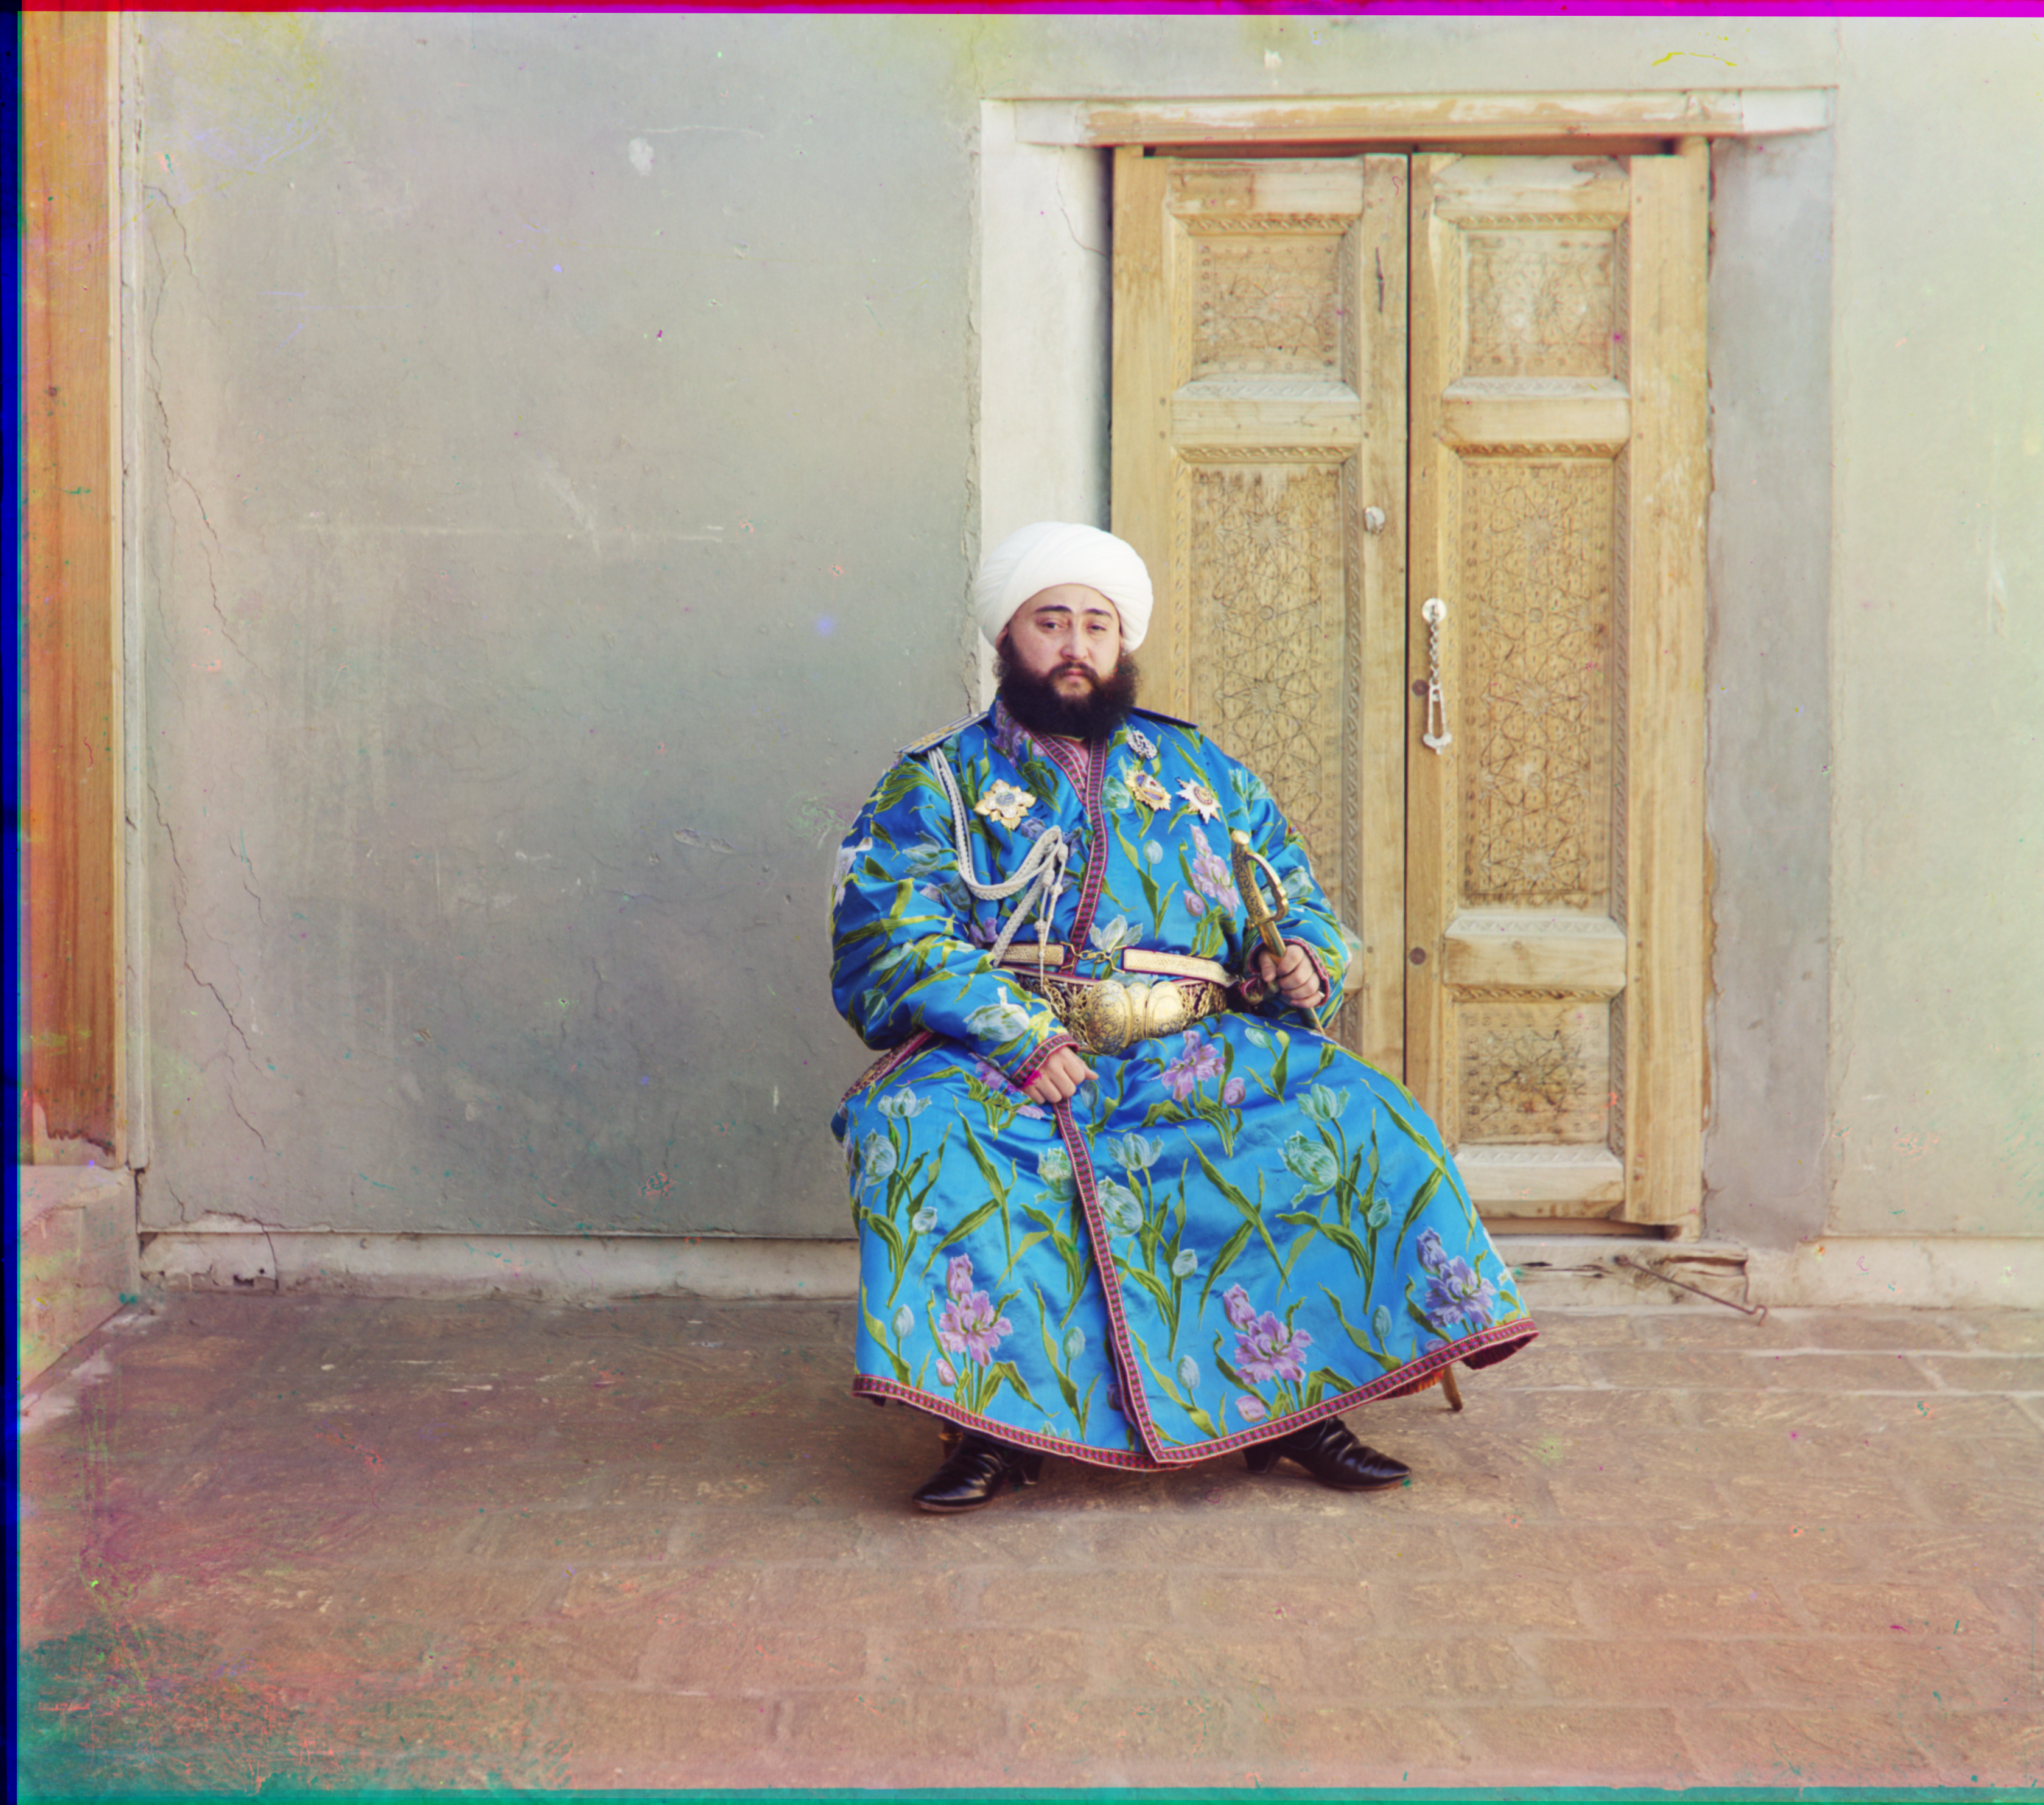
\includegraphics[scale=0.07]{../00152a/composite}
\end{figure}

\FloatBarrier

The Emir of Bukhara. There quite a bit of shift in the red and green images. Again, these are elimated in the SURF alinged image. 

\begin{figure}[!htb]
\caption{Rough Composite 00223a}
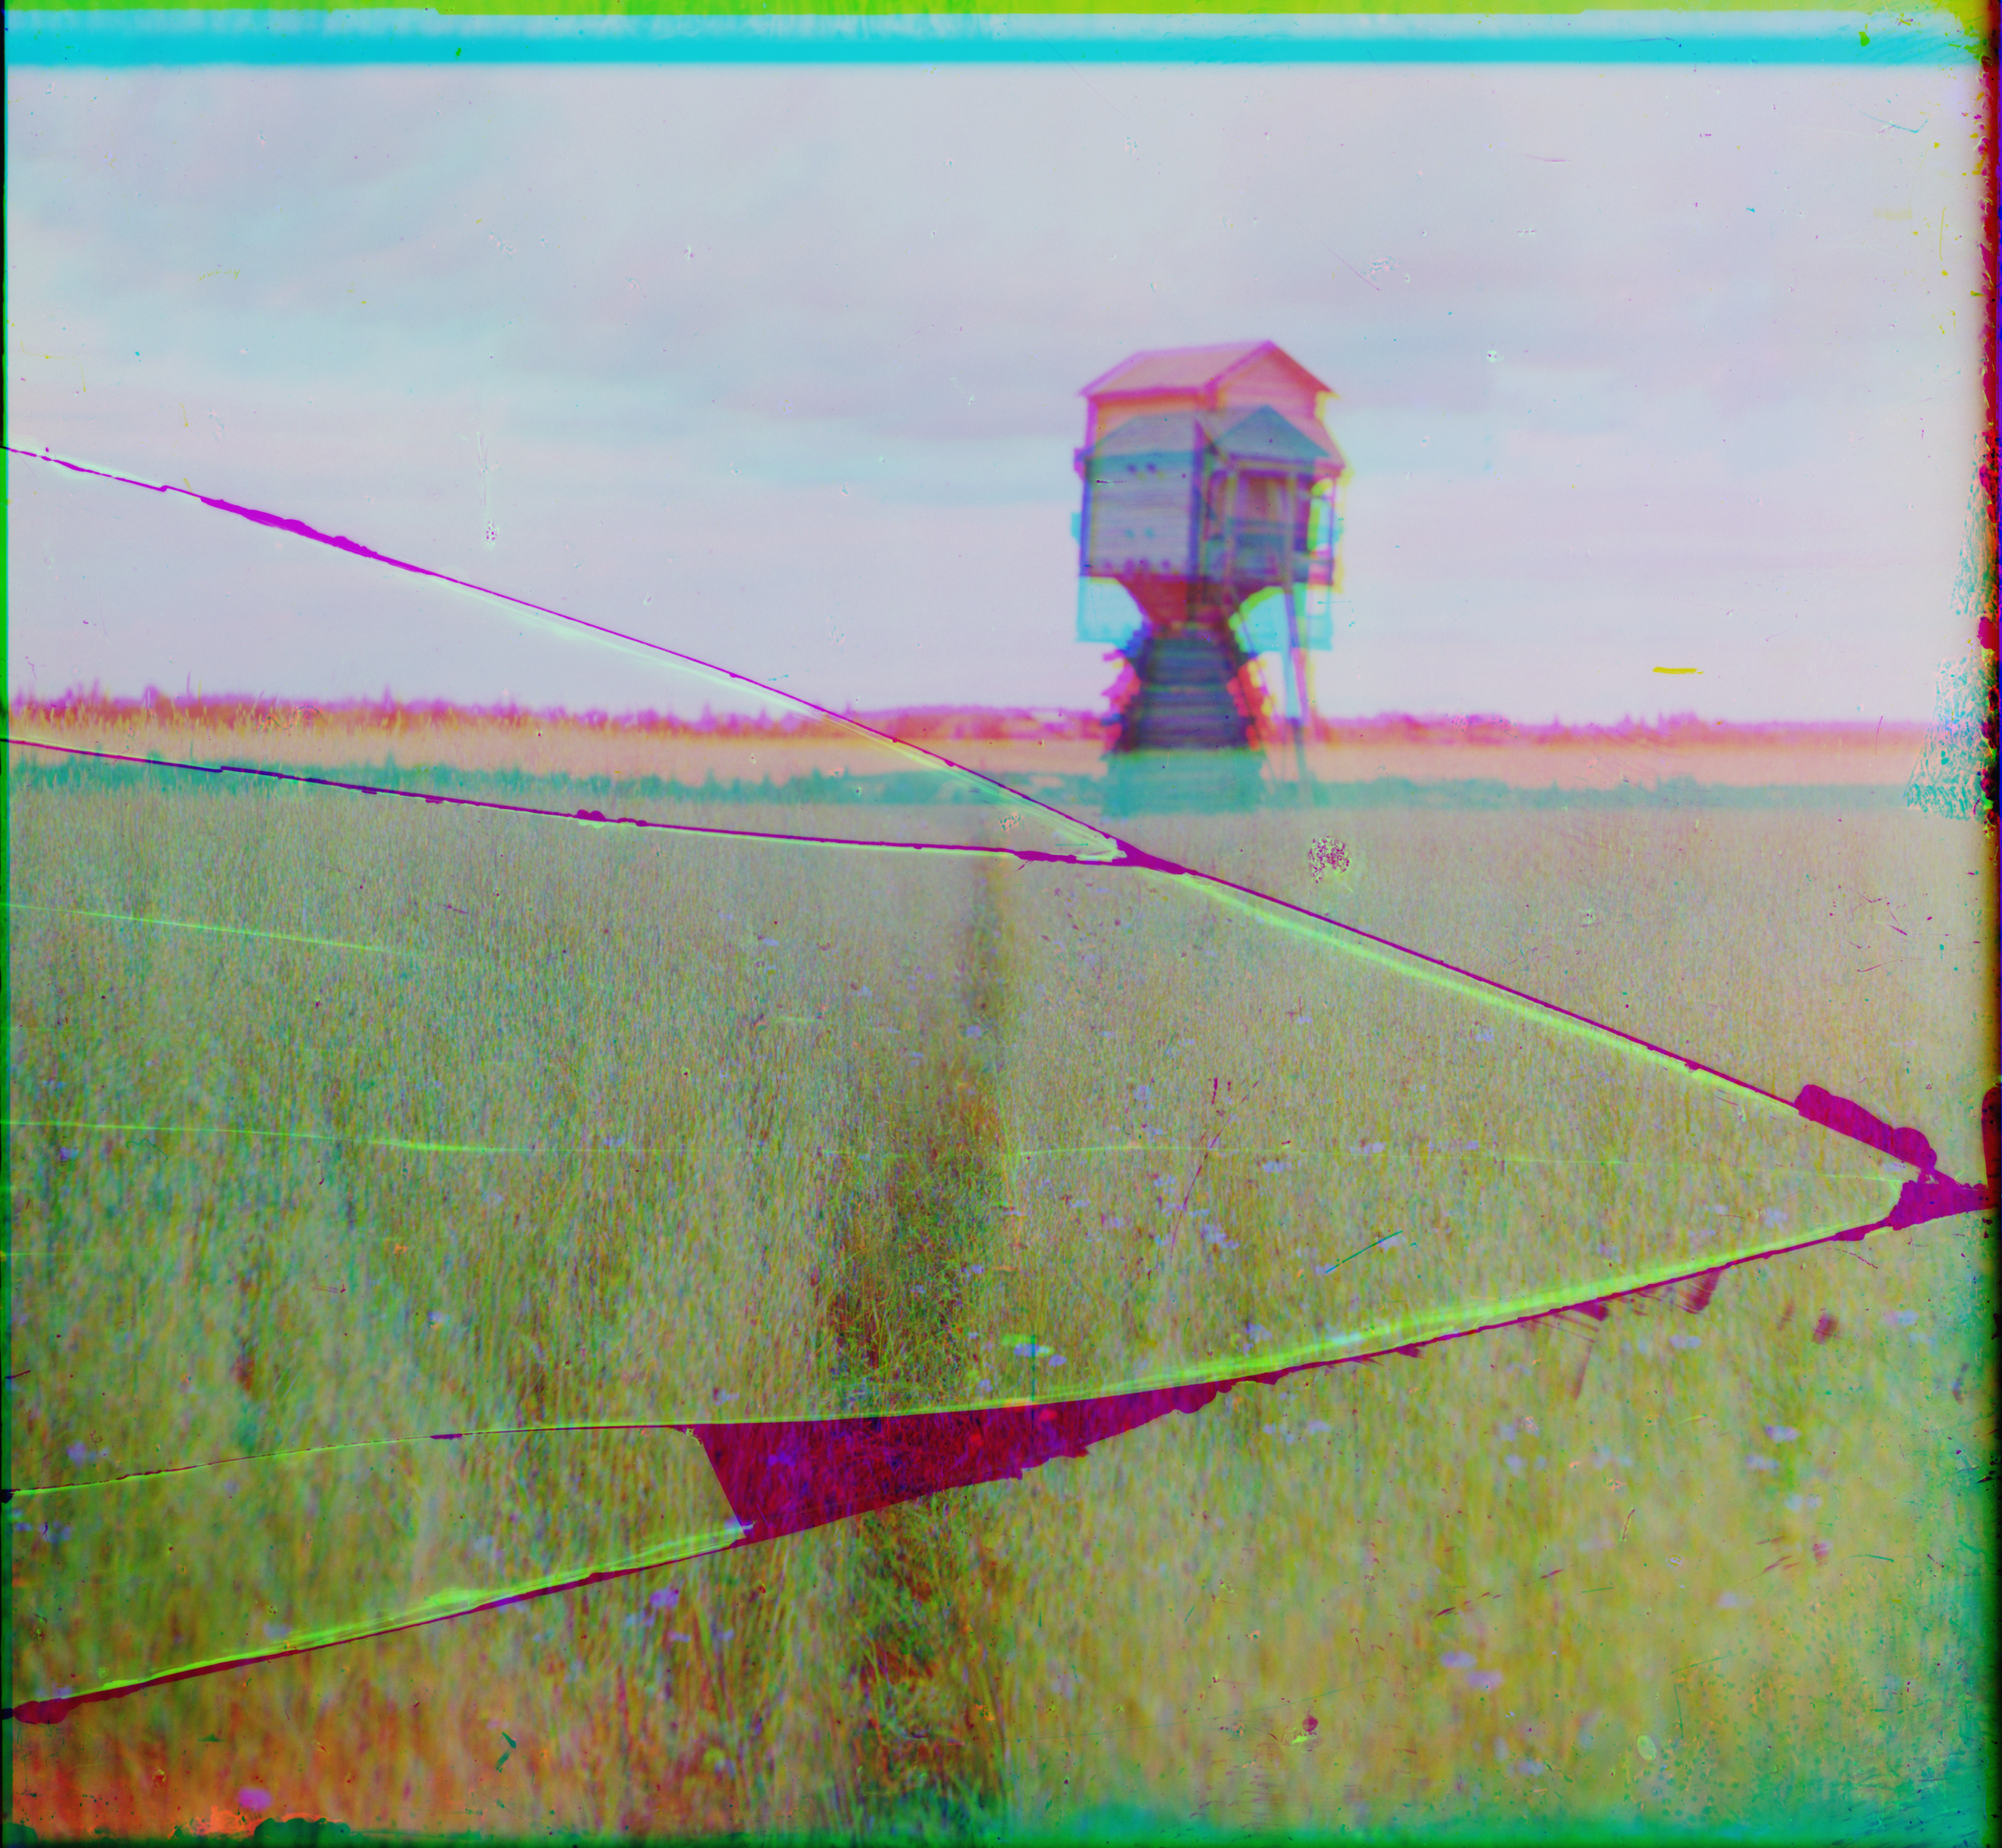
\includegraphics[scale=0.07]{../00223a/original}
\end{figure}

\begin{figure}[!htb]
\caption{SURF Aligned Composite 00223a}
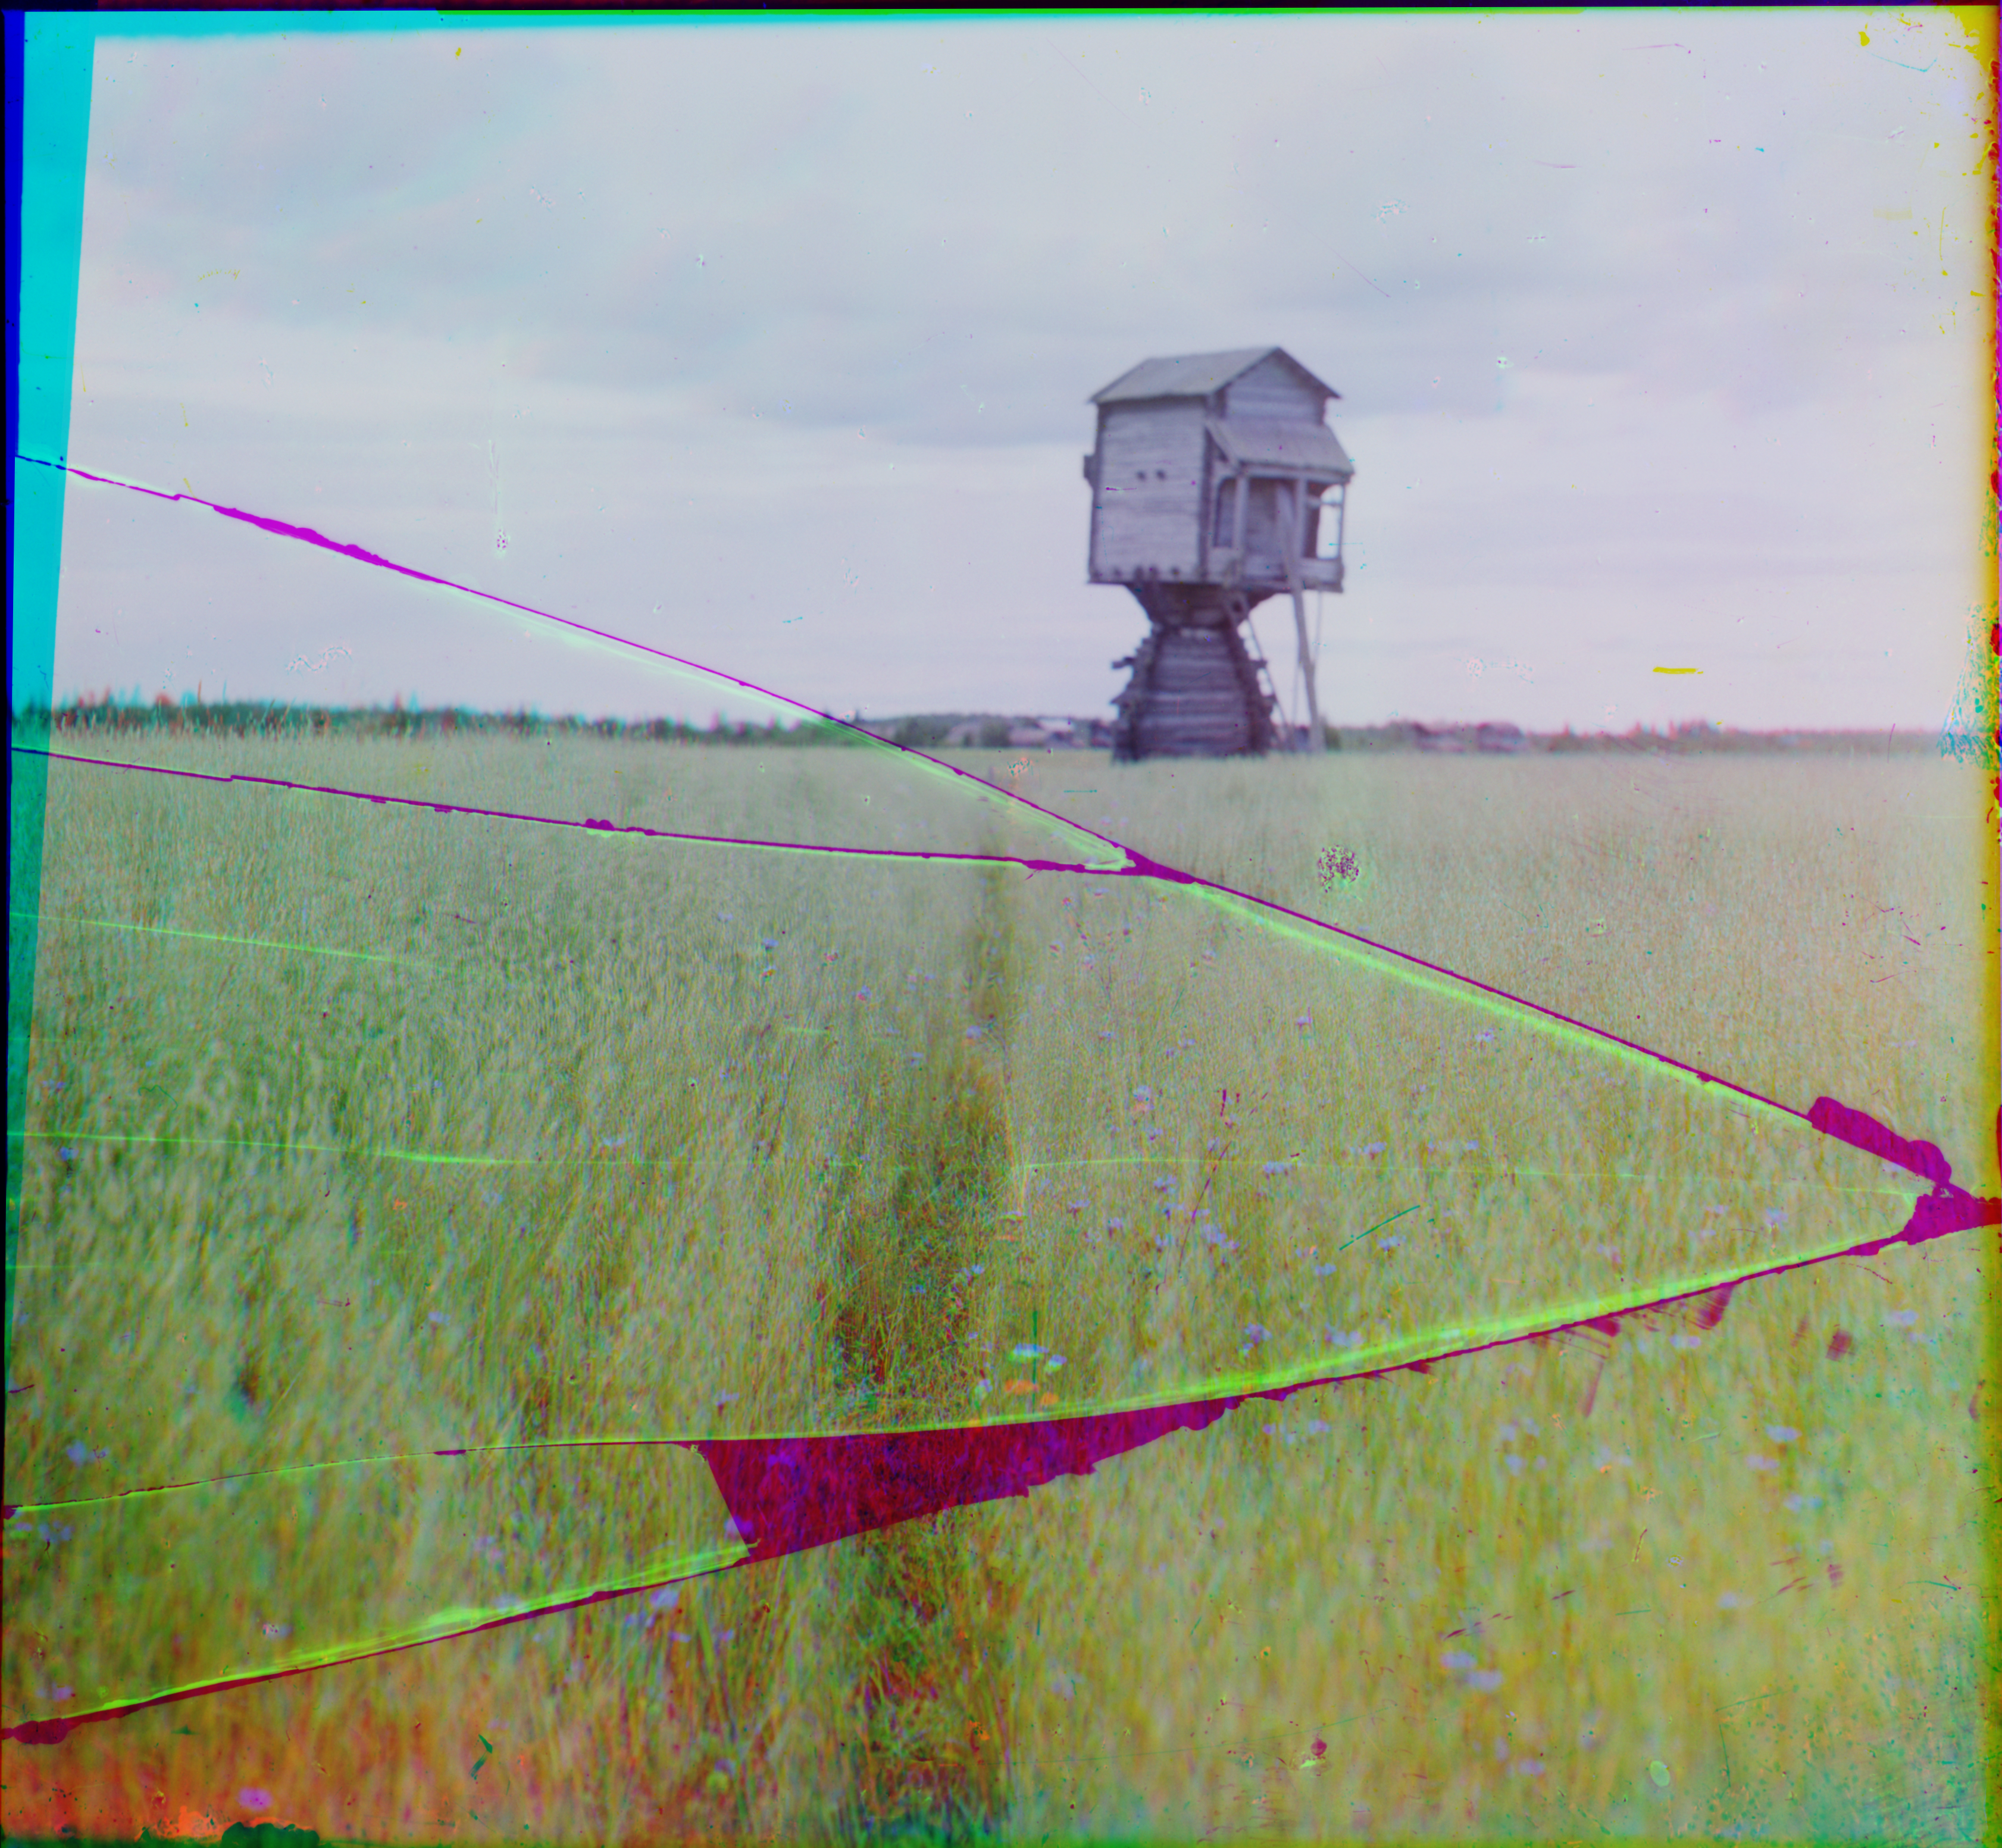
\includegraphics[scale=0.07]{../00223a/composite}
\end{figure}

\FloatBarrier

The negative for the green image is very damaged. There is also a lot of shift with all three colours. The alogrithm lines up the grain silo well, but the grass and flowers in the foreground are still shifted quite a bit. 


\begin{figure}[!htb]
\caption{Rough Composite 00026a}
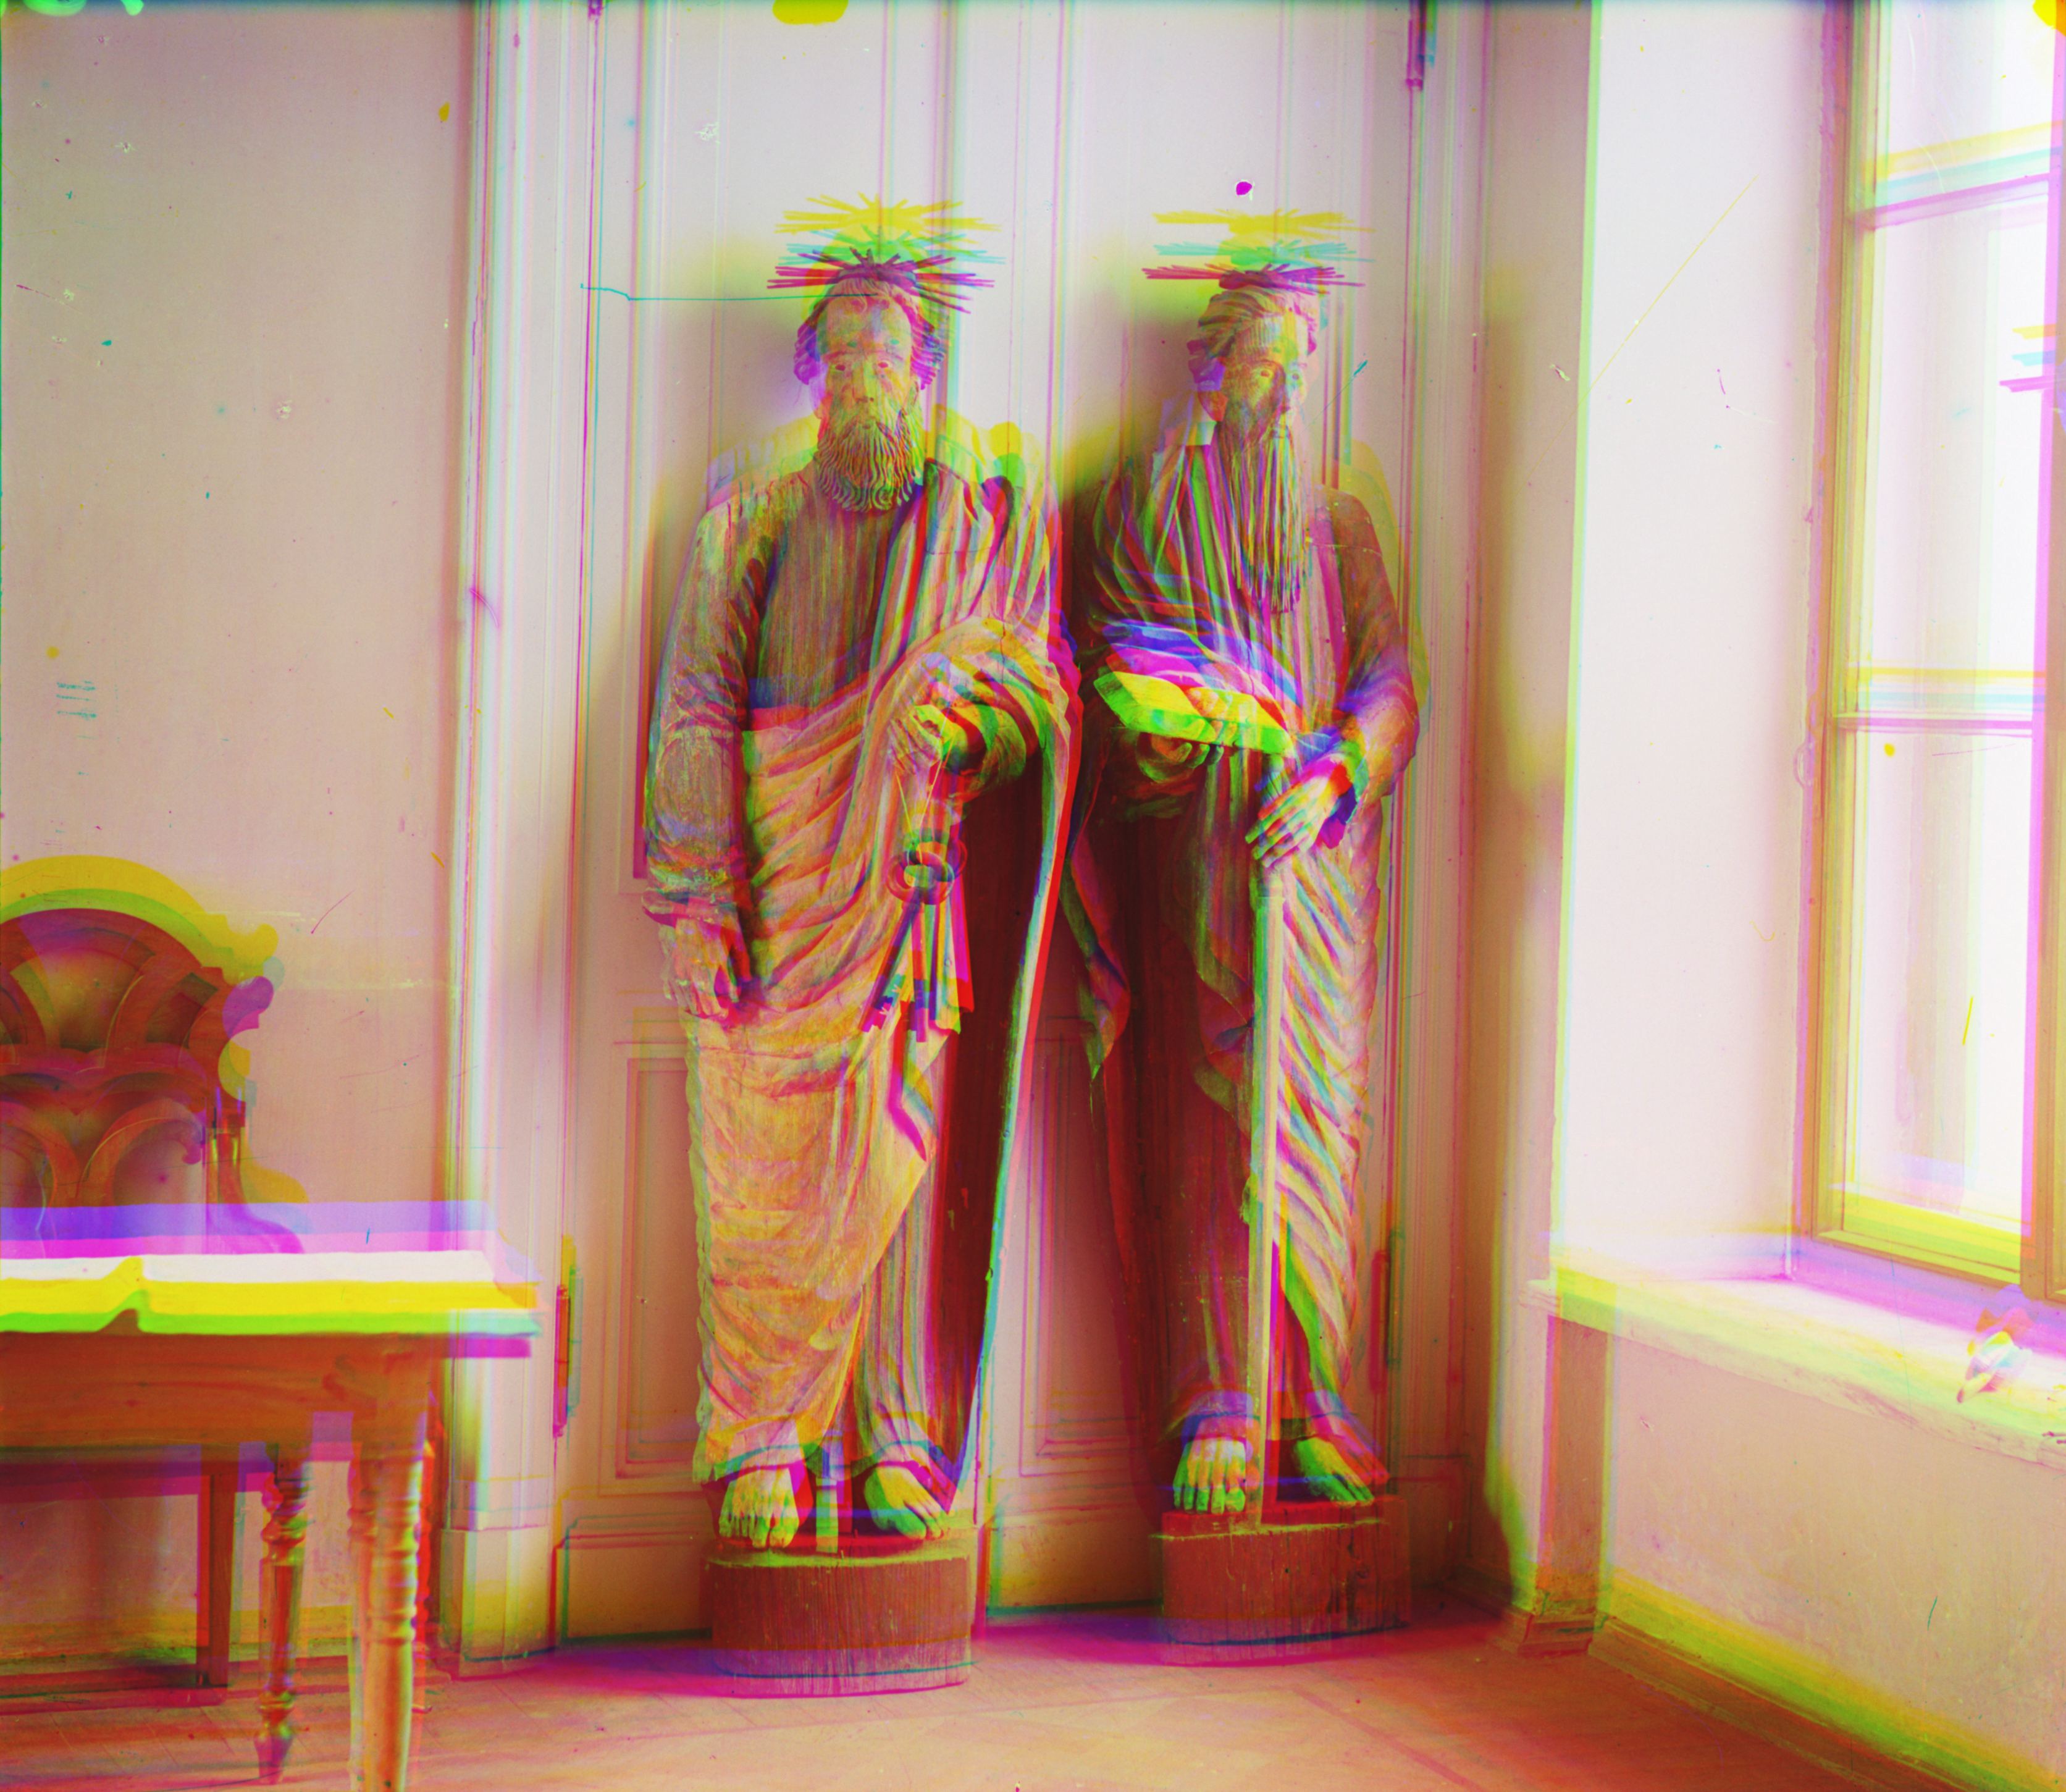
\includegraphics[scale=0.07]{../00026a/original}
\end{figure}

\begin{figure}[!htb]
\caption{SURF Aligned Composite 00026a}
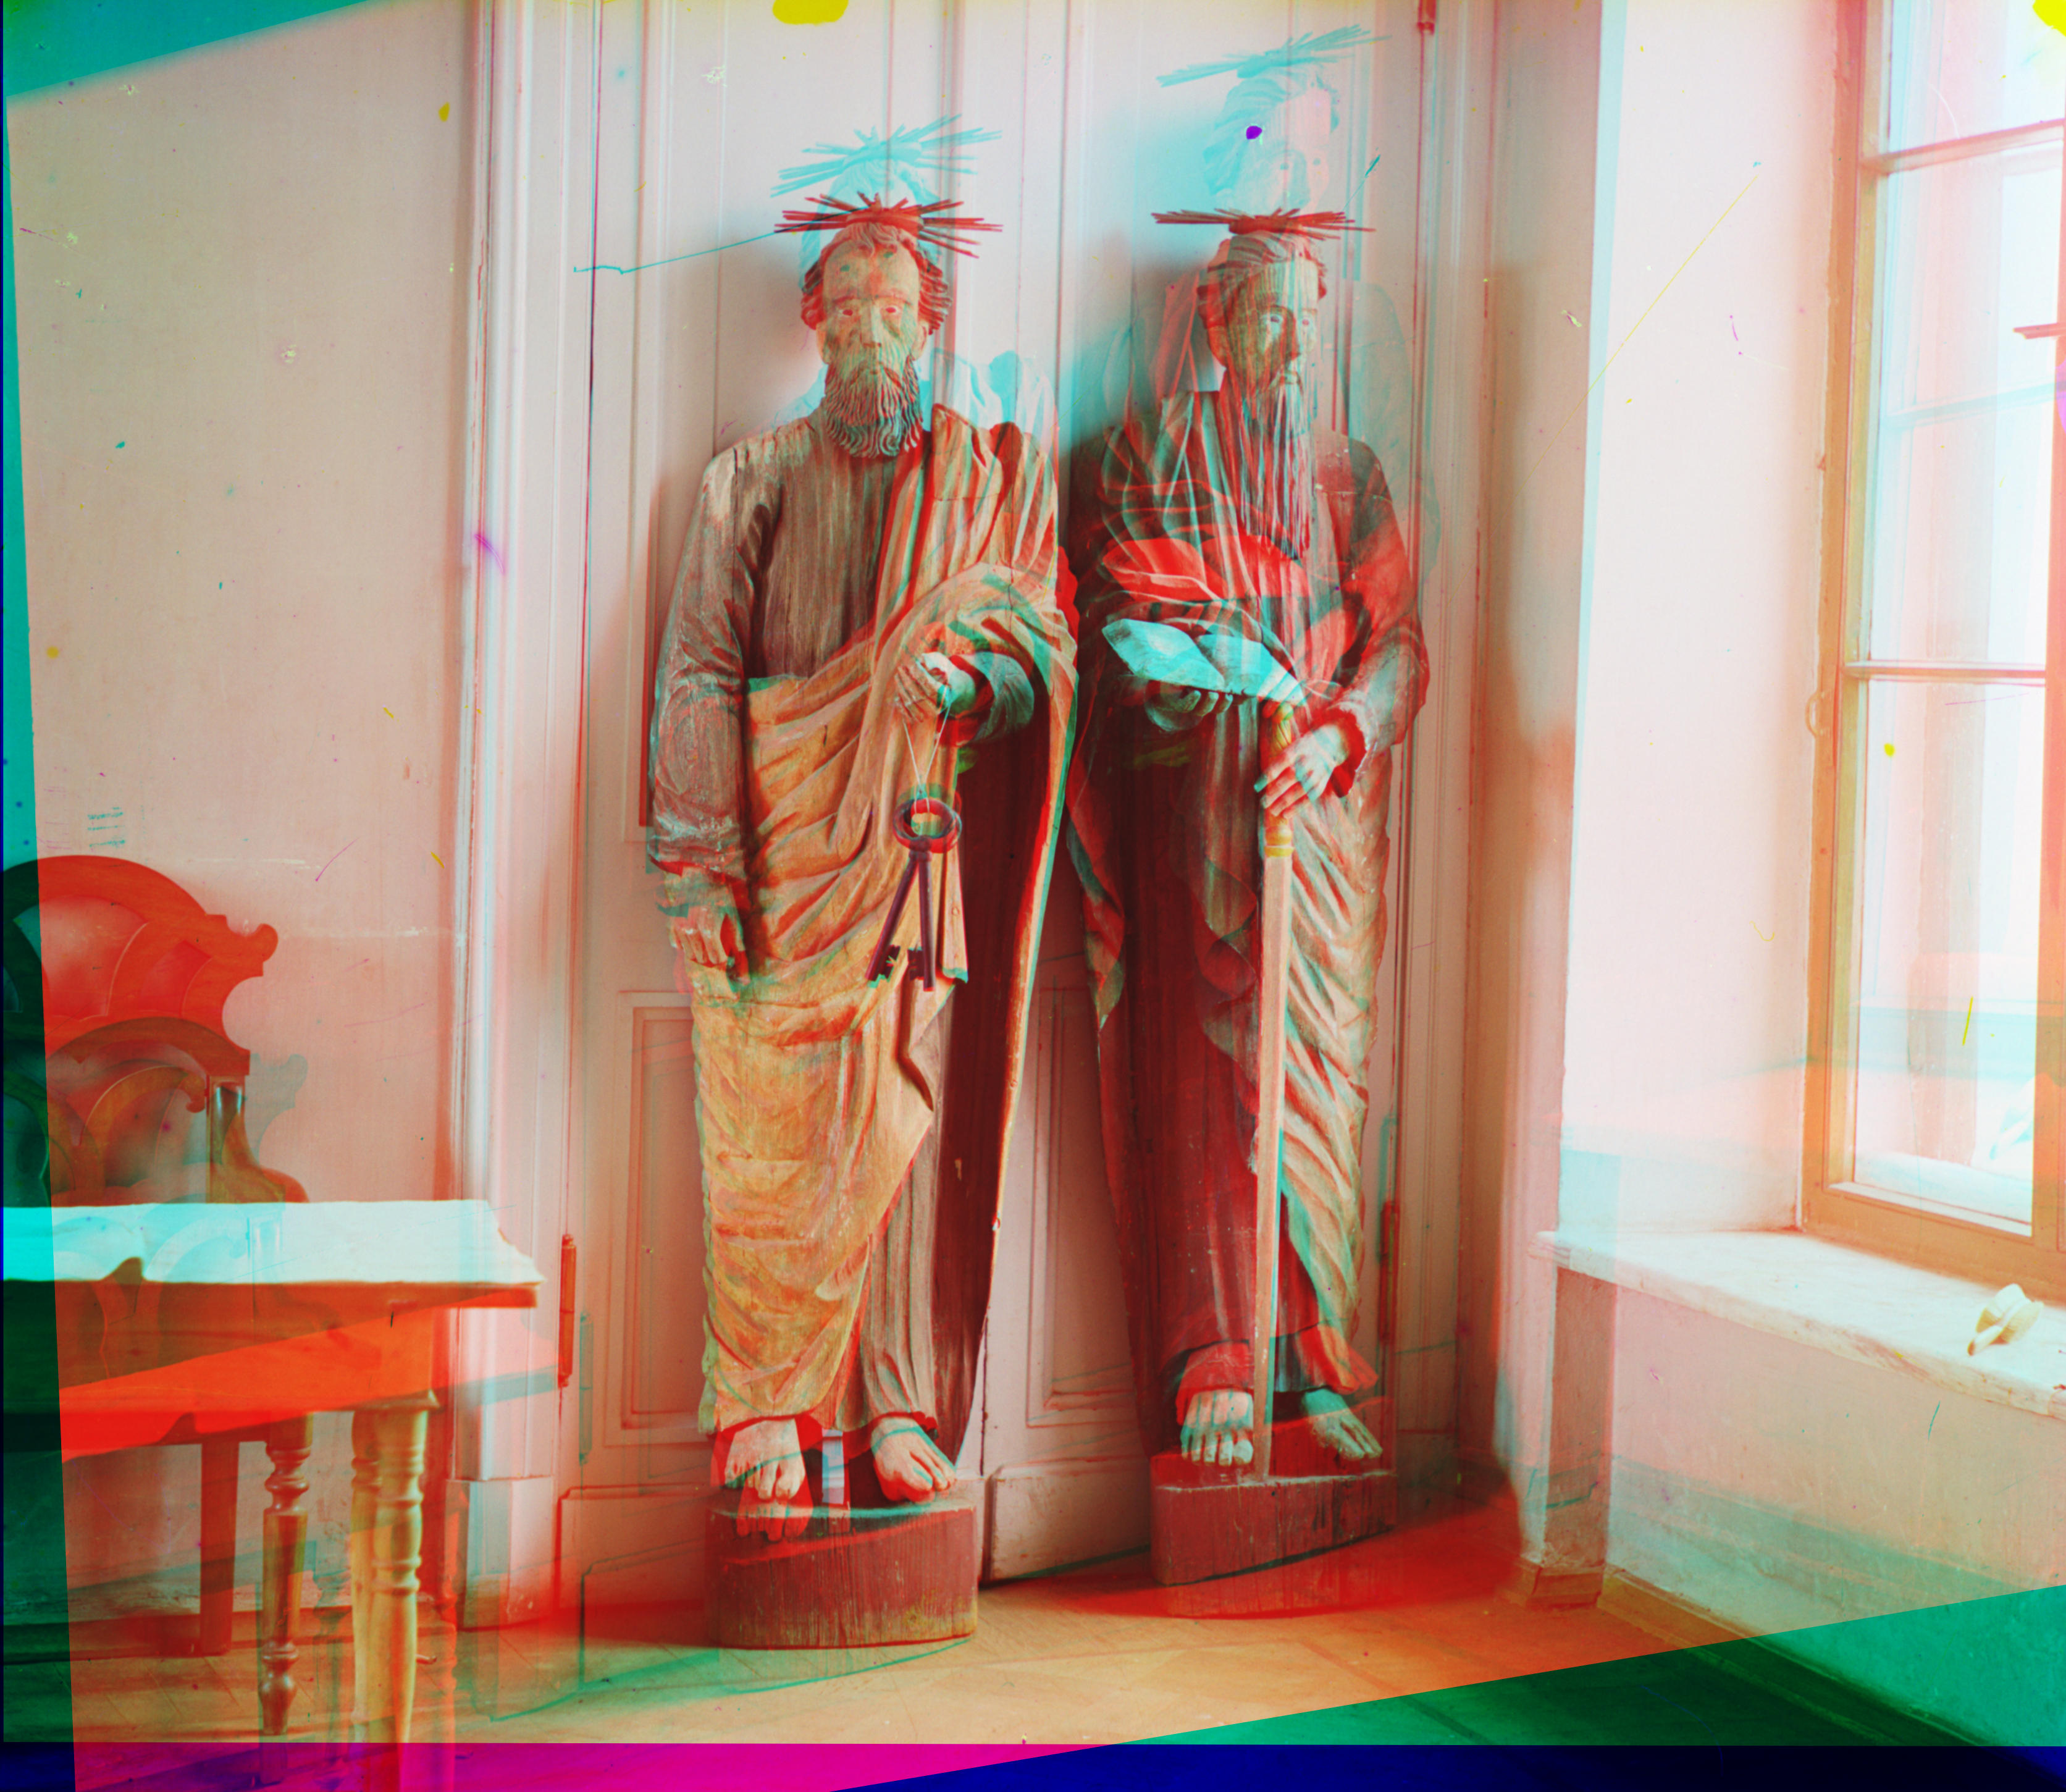
\includegraphics[scale=0.07]{../00026a/composite}
\end{figure}

\FloatBarrier
There is a considerable angle in the red image, as the perspective warpper tried and failed to realign based on the homograph built using the output of SURF. This is likely due to missing keypoints caused by the distance threshold of 10\%. Adjustments to this threshold can cause wildly different results. Increasing it to 25\% will aloow this image to process correctly, but will cause other images to begin failing.  SURF may be matching keypoints that are not acutally the same feature in the image or keypoints may genuinely be greater than that distance away from each other.   

\begin{figure}[!htb]
\caption{Rough Composite 00384a}
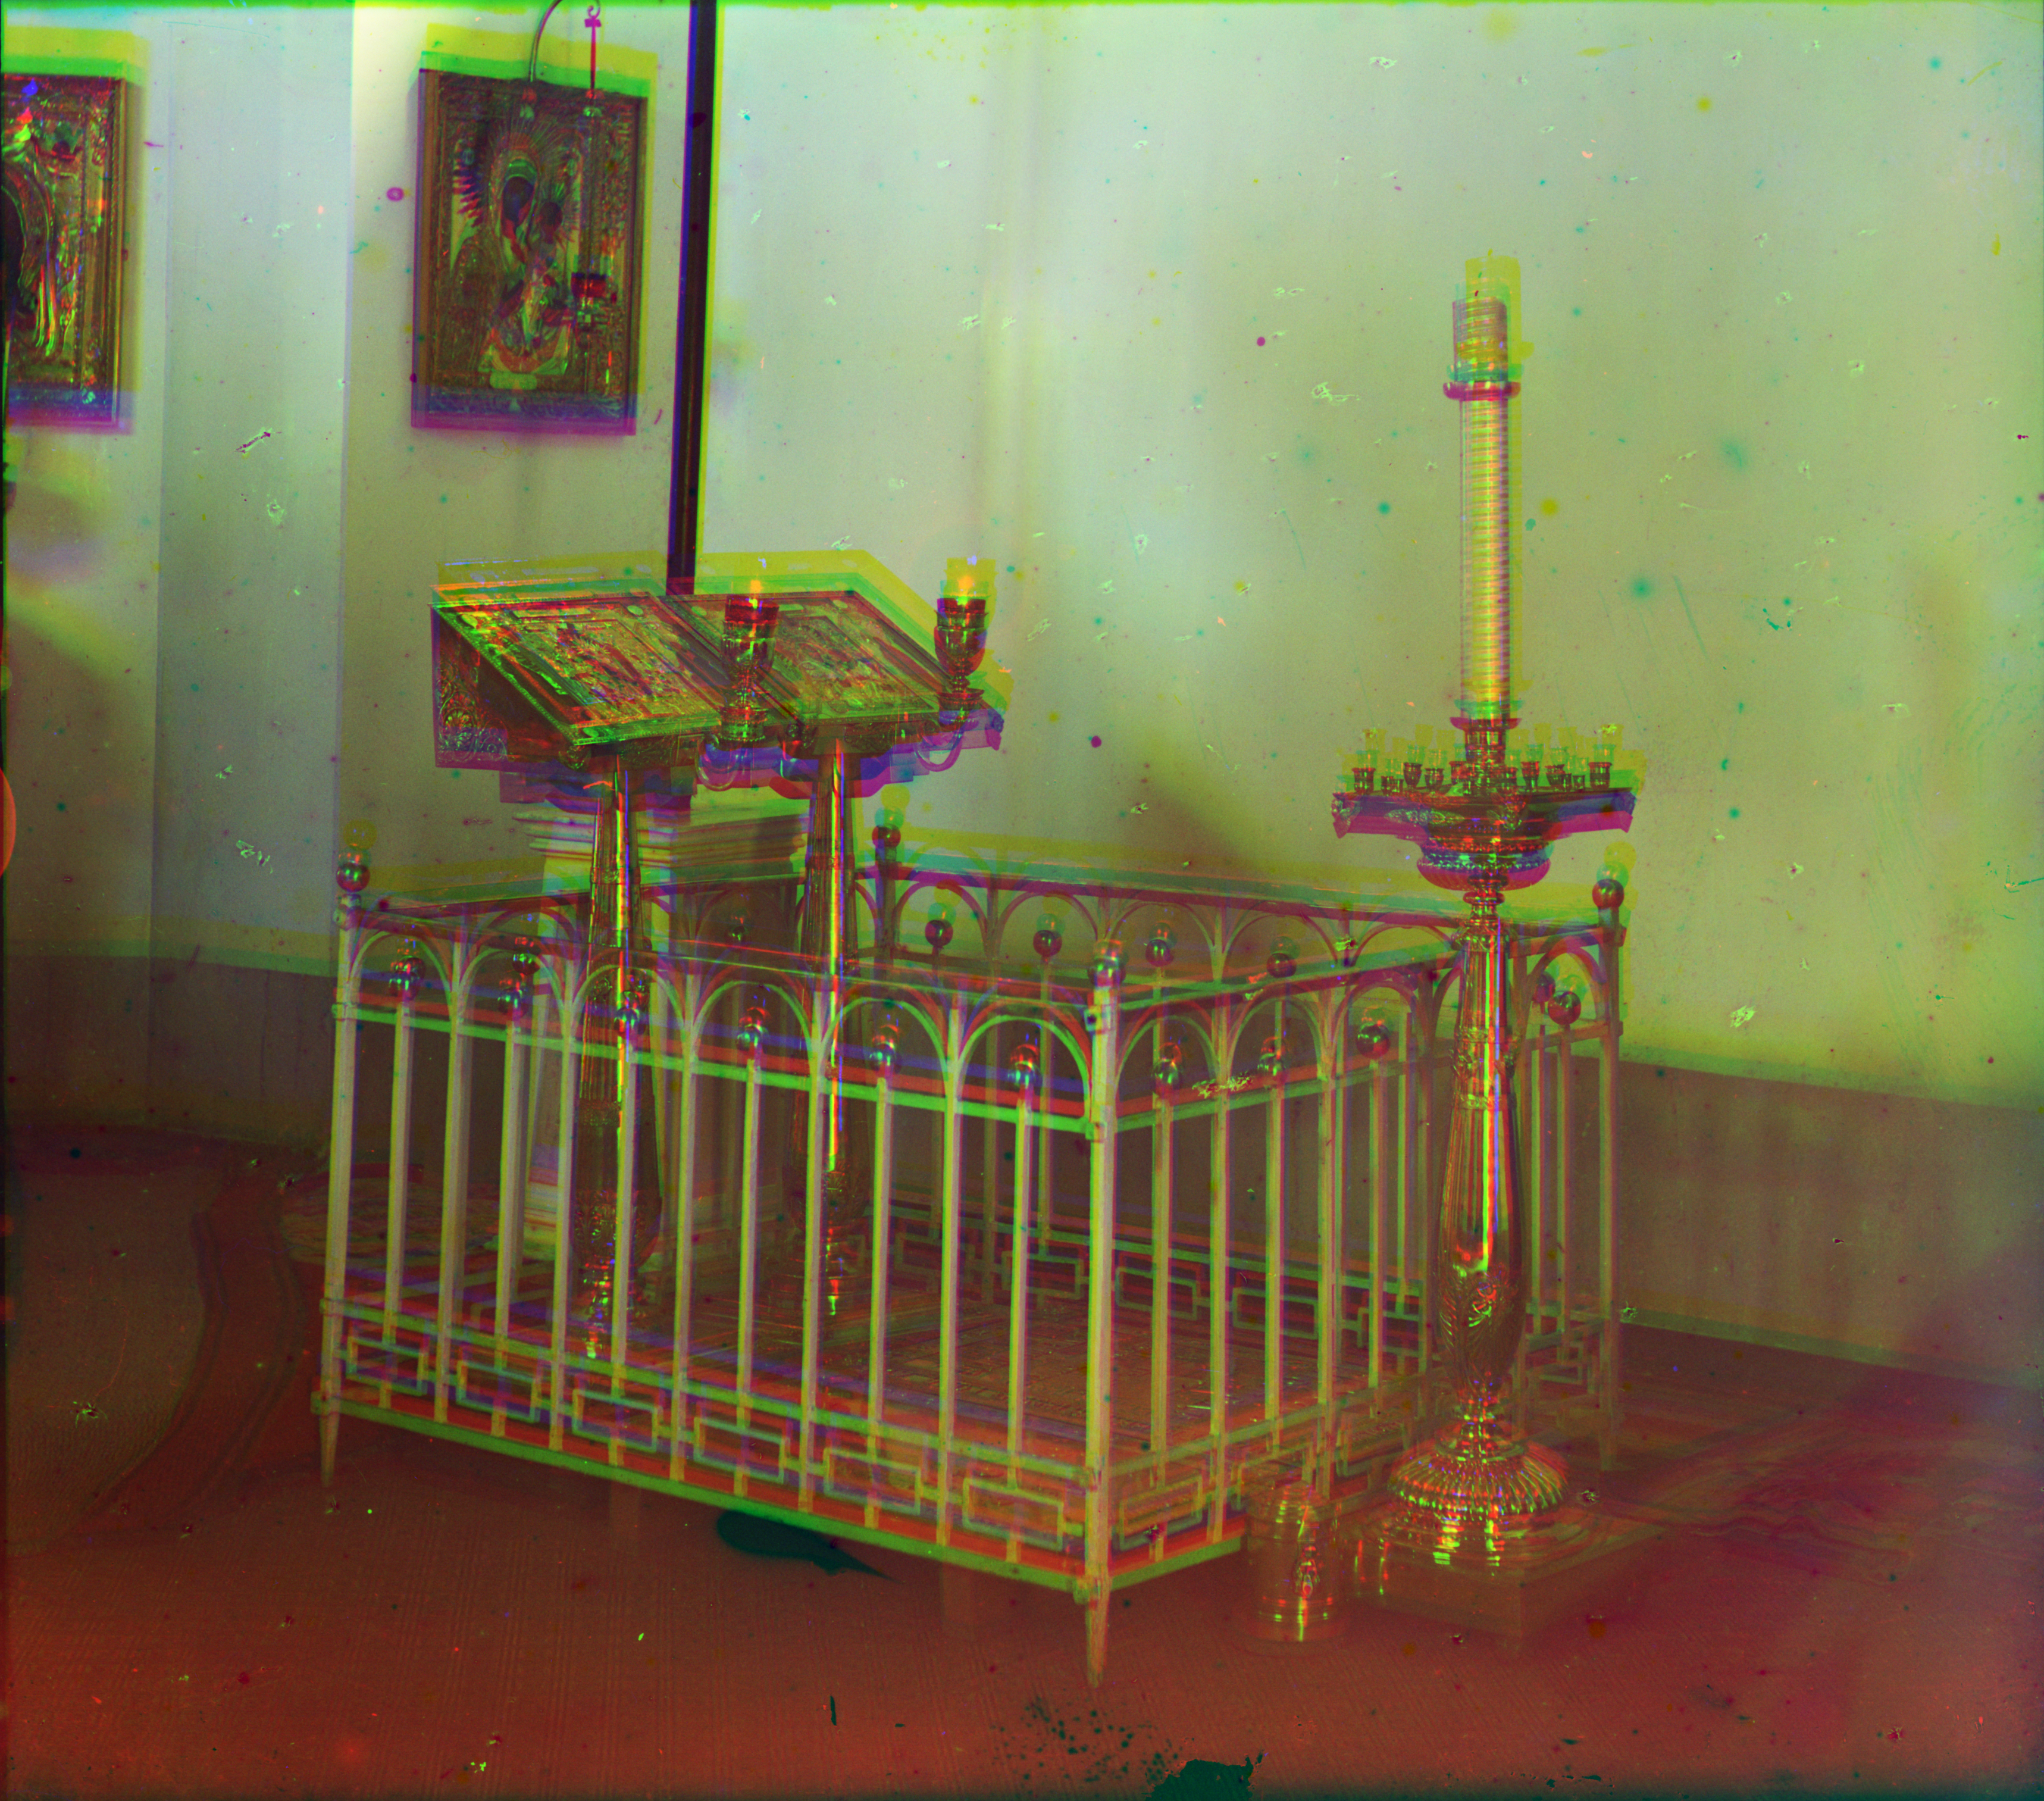
\includegraphics[scale=0.07]{../00384a/original}
\end{figure}

\begin{figure}[!htb]
\caption{SURF Aligned Composite 00384a}
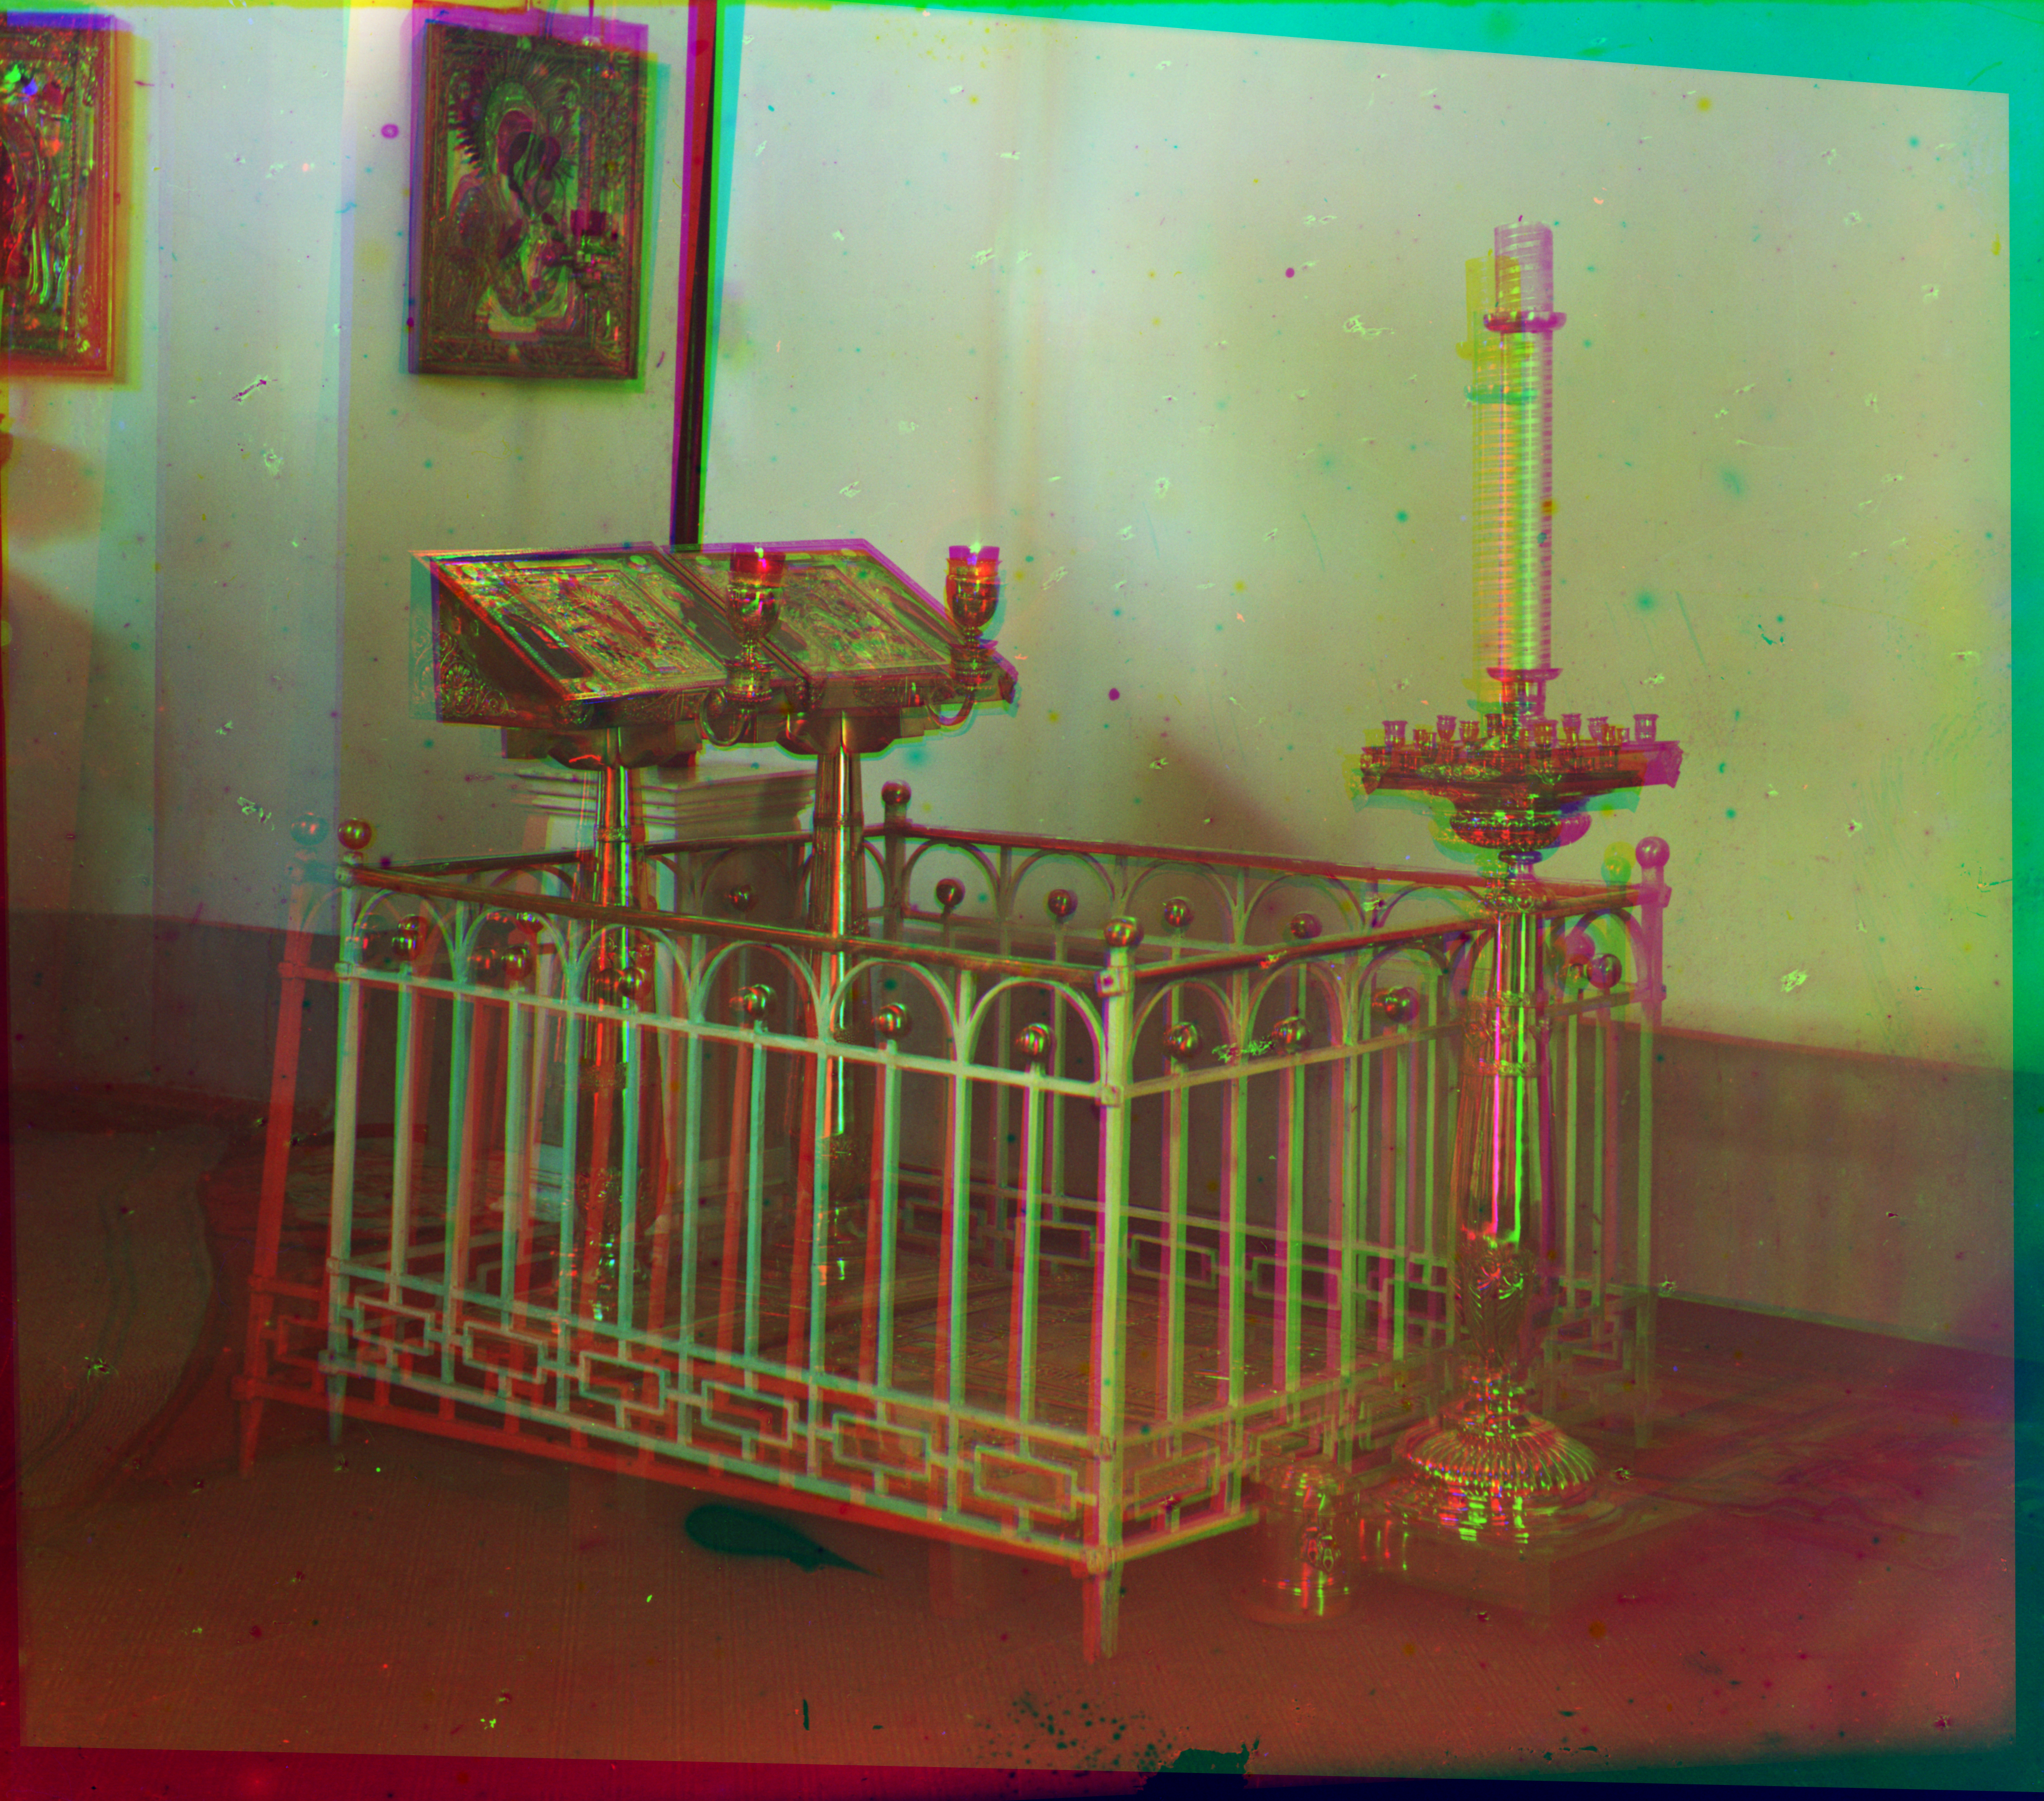
\includegraphics[scale=0.07]{../00384a/composite}
\end{figure}

\FloatBarrier

Second image with the same failed results as 00026a, and likely for the same reasons as well.

\newpage

\section{Conclusion}

Along with 00026a and 00384a, two other images failed, for a success rate of 61 out of 65. Many of the success are better than others, but generally SURF a good job at identifying features and building descriptors with which the rest of the code can acurately line up the colour images. The distance threshold used to filter matches is definitely a number that can be experimented and adjusted more to see if an ideal value can be determined. 



		

%	Uncomment this when there's actually some references
%	It expects references.bib
%	\bibliographystyle{IEEEtran}
%	\bibliography{IEEEabrv,references}
\end{document}
